\documentclass[10pt]{article}
\usepackage[utf8]{inputenc}
\usepackage[T1]{fontenc}
\usepackage{amsmath}
\usepackage{amsfonts}
\usepackage{amssymb}
\usepackage{mhchem}
\usepackage{stmaryrd}
\usepackage{graphicx}
\usepackage[export]{adjustbox}
\graphicspath{ {./images/} }

\title{Introduction to Water Distribution Systems }

\author{}
\date{}


\begin{document}
\maketitle
\section{What Is In This Chapter?}
\begin{enumerate}
  \item Functions of a distribution system

  \item Types of distribution systems

  \item Common distribution piping materials

  \item Common distribution system fittings

  \item Major components of piped systems

  \item Distribution system pipe installation

  \item Common household service equipment and materials

  \item Common reservoirs and their components

  \item Typical utilidor components and operation

  \item Basic operation and maintenance requirements of a distribution system

  \item Common methods to control cross connections

\end{enumerate}
Key Words

\begin{itemize}
  \item "C" Factor

  \item Air Gap

  \item Altitude Valve

  \item Appurtenances

  \item AWWA

  \item Backflow

  \item Backsiphonage - Butterfly Valve

  \item Compression Hydrant

  \item Cross Connection

  \item Double Check

  \item HDPE

  \item Hydrant Bury

  \item Invert - Mechanical Joint

  \item MVO

  \item NSF

  \item Peak Demand

  \item PVC

  \item Reservoir

  \item RPZ - Seal Water

  \item Slide Gate Hydrant

  \item Thrust Block

  \item Toggle Hydrant

  \item Vacuum Breaker

  \item Water Hammer

\end{itemize}
\section{Introduction}
\section{Lesson Content}
This lesson on the introduction to distribution systems is focused on the description of the various components of a distribution system, their function, and their purpose. Some details on the proper operation and maintenance of components in a distribution system are covered here, but you may want to consult additional manuals for a more detailed discussion.

\section{Cost Factors}
In most communities, the water distribution system is their largest single capital investment. To preserve this investment, careful attention should be paid to the proper operation and maintenance of the system. This starts with a good understanding of the components and their function.

\section{Primary Function and Design}
The basic function of a water distribution system is to transport the water from the treatment facility to the customer. In addition, distribution systems may also provide storage, as well as provide flow and pressure adequate for fire protection. Typically, the size of water mains, pump station capacity, and storage reservoir volume is determined by fire suppression needs. The volume of water necessary to fight fires is much greater than domestic and commercial water demand in most communities.

\section{System Criteria}
To provide this basic function in a proper manner, criteria have been established for distribution systems. Distribution systems should provide adequate and reliable water to the customer. Adequate means providing all the water the customer needs at a pressure not less than 20 psi. Adequate also means that the water provided meets the customer's needs for quality. Reliable means that customers can expect to obtain all the water they need, anytime they need it. In other words, they can expect that there will be water at the tap. As part of being adequate and reliable, the system must be operated in a way so that the quality of the water does not deteriorate between the treatment facility and the customer.

In many communities, the customer expects that adequate reserves are present for fire prevention. If there are fire hydrants on the system, the customer has every right to make this assumption, and the purveyor has the responsibility for meeting this expectation by providing adequate flow, pressure, and storage volume.

\section{Types of Systems}
In many villages in Alaska and Canada, watering points substitute for a normal distribution system. These are systems with one or more specific points in the village where the customer can obtain water. This is the modern version of the community well. In some villages, there is a combination circulating system and watering points. The watering points are used by those customers who have homes away from the piped system.

Another type of system found in Alaska and Canada is the haul system. With the haul system, water is delivered using a truck and tank or a snow machine and tank. The water is delivered on order in much the same manner as fuel oil is delivered. The most traditional water distribution system is the piped system. There are two types of piped systems: the conventional system and the completely looped circulating system. The circulating system is common in the arctic.

\section{Review}
\begin{enumerate}
  \item List the three primary functions of a water distribution system.

  \item What are the two criteria for a water distribution system?

  \item The pressure in a water distribution system should never drop below psi.

\end{enumerate}
\section{Watering Point System}
\section{Description}
A watering point is a location in a village where customers can access the water supply. In some villages, the only source of water for customers is from the watering point. There may be more than one watering point in the village, depending on its population.

\section{Treatment}
The treatment process for a watering point system is the same as for a piped system.

\section{Equipment}
A storage reservoir may or may not be necessary for a watering point system, depending on source production. The reservoir may be close to or inside the treatment plant. Standard reservoir designs are used in these systems. The reservoirs may be steel, concrete, or wooden gravity tanks or steel hydropneumatic systems.

When the watering point is near or adjacent to the treatment plant, the piping material used is the same as would be used in the treatment plant; copper, galvanized steel, $\mathbf{P V C}^{1}$, and $\mathbf{H D P E}^{2}$ are common. When the watering point is away from the treatment plant, the piping material is the standard material used in piped distribution systems for that particular climate.

There are as many methods of obtaining water from the watering point as there are watering points. The most common of these techniques is to use a flexible hose and automatic hose reel. The hose must consist of $\mathbf{N S F}{ }^{3}$-approved material, not a garden hose. In cold climates, reinforced, arctic-grade, heat-traced hose with a PVC liner may be provided. A means of backflow ${ }^{4}$ prevention must be provided to protect the public system from potential contamination.

In some instances, the watering point may contain a coin, key, or coupon-operated dispensing system and a meter. Each coupon will allow a set volume of water to be delivered. The coupon system allows the village to obtain a fair payment for the cost of treating the water, as well as operating and maintaining the watering point.

\section{Haul System}
\section{Description}
A haul delivery system may be supplemented or used in conjunction with a standard piped system, such as in Fairbanks and Barrow, or may be the only means of water being delivered to the customer.

\section{Treatment}
The treatment process for a haul system is the same as for a piped system or watering point.

\section{Equipment}
The most common haul systems use a high-quality tank mounted on a truck or snow machine. The water in the tank is prevented from freezing by using the heat from the engine exhaust system.

The methods used to get water from the truck to the customers holding tank is typically $1 \frac{1}{4}$-inch or larger NSF-approved flexible pipe. In cold climates, a reinforced arctic-grade, heat-traced hose with a PVC liner may be used. Sometimes a dispensing pipe is elevated so that haul trucks can park beneath the water pipe. A means of backflow prevention must be provided to protect the public system from potential contamination.

The delivery tank should be cleaned and disinfected with a chlorine solution similar to the disinfection process used for a reservoir. Hauling tanks should not be used for other purposes such as pesticide or sewage hauling.

\section{Piped Distribution System}
\section{Description}
A piped system can vary from simple to extremely complicated. Most piped systems have the same basic components: pipes, valves, fire hydrants, service connections, and reservoirs. Piped systems may also have pumping stations. The following describes the various components that can be found in a piped system, excluding pumping.

${ }^{5}$ AWWA (American Water Works Association) - An association of waterworks personnel, equipment manufacturers, suppliers, and engineers.

\section{Main Line Piping Materials Gray Cast Iron Pipe (GCIP)}
Gray cast iron pipe used in the waterworks industry is manufactured to meet $\mathbf{A W W A}^{5}$ standard C-106. This is some of the oldest piping material in use today. Over 200 cities in the United States have pipe installed that has been in use for over 100 years. Gray cast iron pipe was first manufactured using a process called pit casting. In this process, the molten iron was poured into a mold and allowed to cool. In 1925, a process called spin casting was developed. In this process, molten iron is injected into a spinning mold. The result is a pipe of consistent diameter and wall thickness.

\section{Ductile Cast Iron Pipe (DCIP)}
Ductile cast iron is not an alloy. It is formed by injecting magnesium into molten cast iron. The treatment changes the carbon structure of cast iron from a flake to a spheri- cal shape. This alteration results in a material of high strength. It can withstand high impacts, both internally and externally; it has great beam strength (won't break easily); and it is much better in resisting corrosion than gray cast iron.

Ductile cast iron pipe is commonly manufactured using the spin cast system. In this process, molten cast iron is injected into either a metal or sand-lined spinning mold. DCIP pipe is available in sizes ranging from three inches to 54 inches and comes in 18-foot and 20 -foot lengths. Lining it with a thin coating of cement mortar enhances the hydraulic capabilities and corrosion resistance of the pipe. Under these conditions, the Hazen and Williams " $\mathrm{C}^{9}$ " Factor $^{6}$ for the pipe is 140.

Ductile cast iron pipe is commonly connected using mechanical joints ${ }^{7}$ (M.J.), flanges or the various common rubber ring push-on joints. Fittings used are commonly made of gray or ductile cast iron and use M.J. or hub joints. Push-on joints are typically used for buried pipe installed below grade because they are quickly assembled and the least expensive. Service taps are made by directly tapping the line or using service saddles.

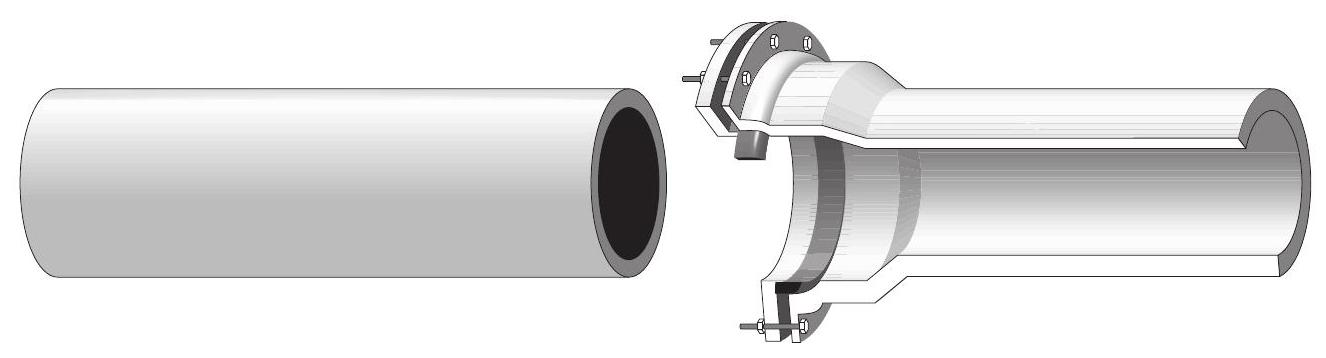
\includegraphics[max width=\textwidth]{MechanicalJoint1}

Mechanical joint\\

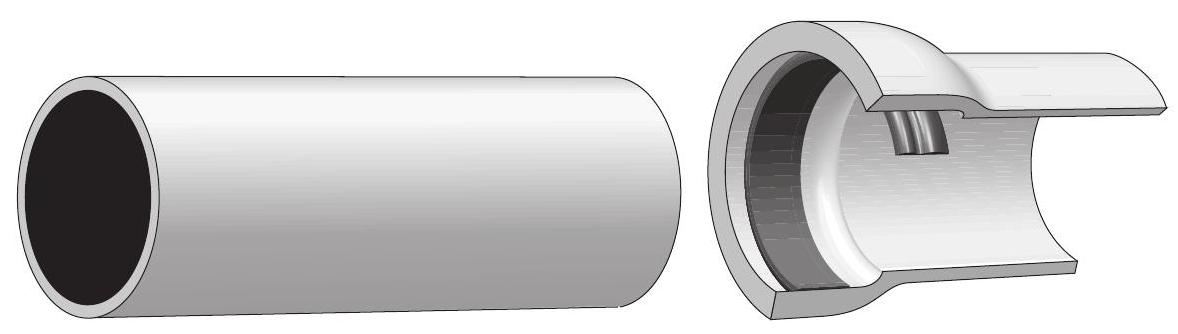
\includegraphics[max width=\textwidth]{PushonJoint1}

Rubber ring push-on joint

\section{Asbestos Cement (A.C.) Pipe}
A.C. pipe is also referred to as Transite ${ }^{\mathrm{TM}}$, which is the trademark of the JohnsManville Corporation, one of the first U.S. manufacturers of the material. The pipe is made by spraying a solution of portland cement, long fibrous asbestos, silica sand, and water onto a spinning anvil. The pipe is then shaped and placed in an autoclave to dry.

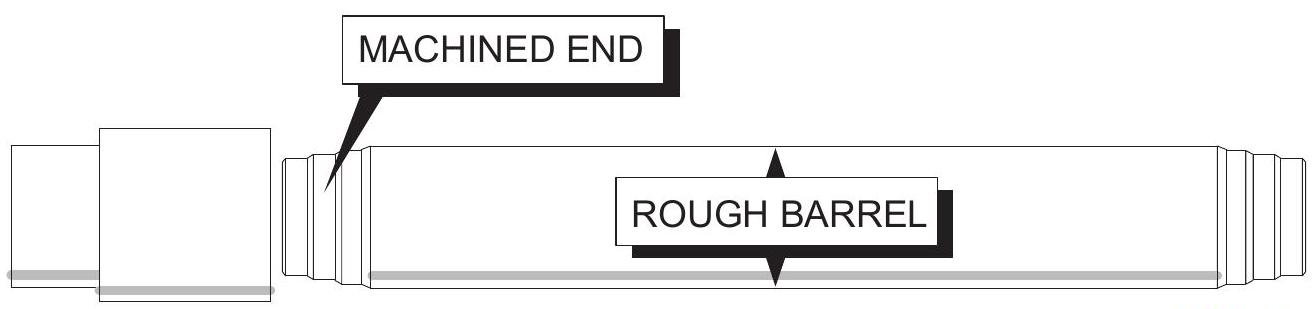
\includegraphics[max width=\textwidth]{2022_11_03_fc0cbc2f3612fab6edd2g-05(2)}

A.C. pipe 6 "C" Factor - The factor used in the Hazen and Williams equation for determining headloss. The "C" Factor is a representation of the hydraulic roughness of the pipe. The larger the number, the smoother the pipe is hydraulically.

${ }^{7}$ Mechanical Joint $-\mathrm{A}$ joint used on cast iron valves, fittings, fire hydrants, and cast iron pipe. The joint consists of a rubber gasket and follower ring held to a flange by a row of bolts. The gasket is compressed between the follower ring and the flange seat. A.C. pipe is available in sizes from three inches to 36 inches and comes in a standard length of 13 feet. There are two common dimensions associated with A.C. pipe. The outside dimension of the pipe itself is referred to as the "rough barrel." The outside dimension where the coupling fits is referred to as the "machined end." To reduce the amount of field machining required during construction, the manufacturers make short sections of pipe that are three feet, three inches and six feet, six inches in length. When the short sections are manufactured similar to the regular pipe, they are referred to as MEE (machined each end). However, short sections are also manufactured with machined end dimensions as the outside diameter. This type of section is referred to as MOA (Machined Over All).

The material is connected together using a double bell coupling with a rubber ring in each end. Fittings and valves used on AC pipe are commonly made of cast iron using a rubber push-on ring for connection. Service line connections may be made by direct tapping of the line or by using a service saddle.

\section{Steel Pipe}
Steel pipe used in the waterworks industry in sizes greater than six inches is manufactured to meet AWWA C-200 standard. Smaller diameter lines used are NSF-approved. These materials may be manufactured by anyone using a variety of means. These materials fall into two categories: mill pipe and fabricated pipe. Typically steel pipe is used in the construction of large-diameter water mains.

Steel mill pipe is available in sizes from $1 / 8$ inch to 36 inches and commonly comes in 21-foot lengths. Two of the most common mill pipes used in the waterworks industry are Standard Weight and Scheduled Pipe. The two common Scheduled Pipes are Schedule 40 and Schedule 80. In sizes from 1/8 inch through 10 inches, standard weight and Schedule 40 pipe are the same OD and wall thickness. From 12 inches through 24 inches, the wall thickness of the standard weight pipe remains constant, while the schedule 40 pipe wall thickness increases with an increase in diameter.

Steel pipe is coupled by a variety of methods: threaded couplings, welded couplings, Dresser ${ }^{\mathrm{TM}}$-type couplings, Victaulic ${ }^{\mathrm{TM}}$ couplings, flanges, and rubber ring push-on joints.

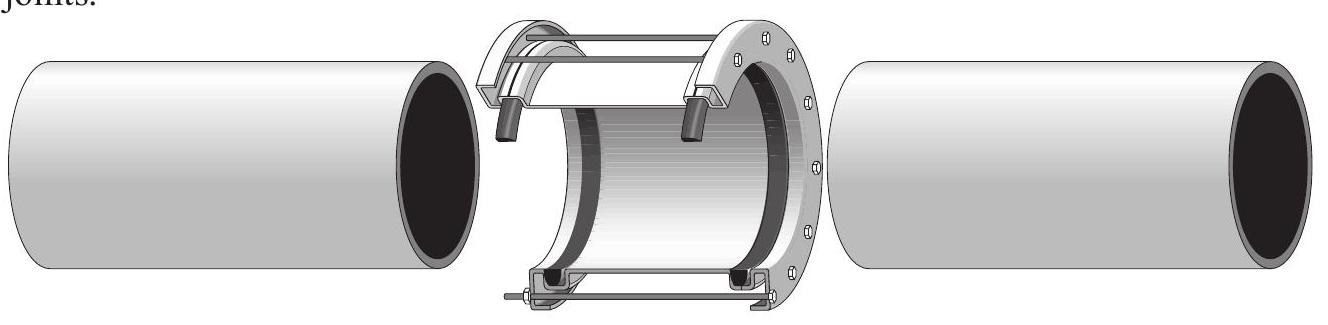
\includegraphics[max width=\textwidth]{DresserCoupling}

Dresser ${ }^{T \mathrm{M}-t y p e}$ coupling

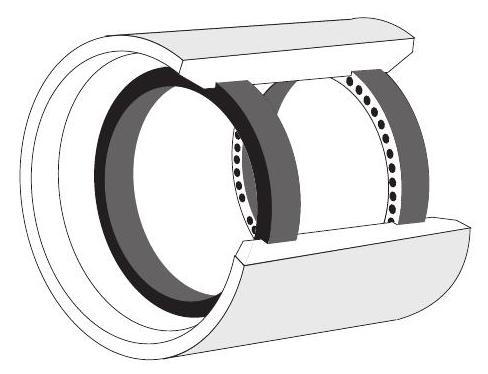
\includegraphics[max width=\textwidth]{DoubleBellCoupling}

Double bell coupling

\section{PVC (Polyvinyl Chloride) PIPE}
PVC water pipe is made from unplasticized polyvinyl chloride. The material is heated and shaped by forcing it through a die in a process called extrusion. Although the material was introduced into the U.S. in the late 1940s, it gained wide acceptance from the larger water systems only when a thicker walled material was developed and an AWWA standard was adopted. The standard that governs most of this thick-walled PVC pipe is called C-900. This distinguishes it from other PVC water pipe that has a thinner wall.

The material is lightweight and easy to install. It is virtually corrosion-free and therefore has gained relatively wide acceptance as a major pipeline material. One disadvantage to PVC pipe is installation in contaminated soils, where fuel oils, gasoline, and other organic compounds may permeate the pipe wall.

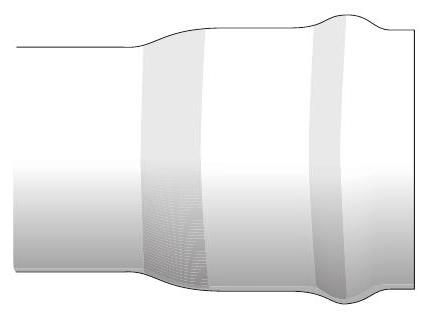
\includegraphics[max width=\textwidth]{PVCIntegralBellSpigotJoint}

PVC integral bell and spigot joint

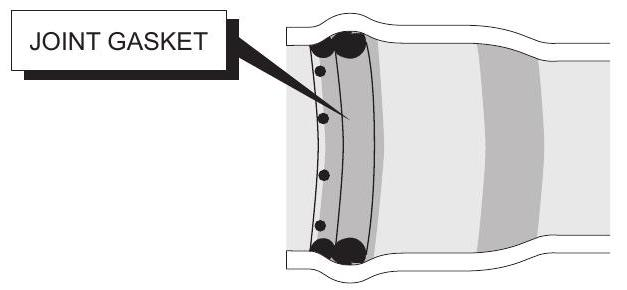
\includegraphics[max width=\textwidth]{PVCIntegralBellSpigotJoint1}

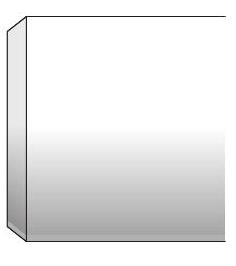
\includegraphics[max width=\textwidth]{PVCIntegralBellSpigotJoint2}

PVC integral bell cross section

PVC used for water lines is generally available in sizes of $1 / 2$ inch through 16 inches. There are three common types of PVC used:

\begin{itemize}
  \item Schedule pipe

  \item Pressure pipe

  \item Class pipe

\end{itemize}
The chief differences among these various pipe types are wall thickness, outside diameter, and burst strength.

Schedule pipe is available in sizes from $1 / 8$ inch through 24 inches, Pressure pipe is available in sizes from $1.5$ inches through 12 inches, and Class pipe is available in sizes from four inches through 12 inches. All three types are available in standard 20-foot lengths. PVC pipe has a Hazen and Williams " $\mathrm{C}$ " factor of 150 . PVC pipe is available in various wall thicknesses and outside diameters. This has resulted in considerable confusion about which pipe is which. In the discussion below, we offer some clarification.

PVC Class and Pressure pipe can be connected using either an integral bell and spigot process or a double-ended bell. In either case, the gasket is a rubber material, and the joints are made by lubricating the pipe and pushing it into the coupling or bell.

\section{Concrete Pipe}
Concrete pipe used in the waterworks industry is manufactured in accordance with AWWA standards C-301 and C-302. This piping material is used primarily for largediameter lines. Several types of concrete pressure pipe are used; however, the most common types of concrete pipe used are manufactured by wrapping a wire around a steel cylinder and using a cement coating to cover the steel cylinder both internally and externally. Concrete cylinder pipe is also available in various prestressed forms. The prestressed pipe is made similar to the pretensioned, except the wire wrap is much smaller and under much higher tension (up to $170,000 \mathrm{psi}$ ). This material is usually used only on large-diameter lines, commonly 36 inches to 240 inches.

One of the most common concrete pressure pipes is referred to as pretensioned concrete cylinder pipe. (A cross-section of this pipe is shown below.) This pipe starts from a steel cylinder. The cylinder is wrapped with a steel rod that is under tension. The interior and exterior of the pipe is coated with cement mortar. The cement is then cured in an autoclave. Concrete cylinder pipe is an extremely durable material with high hydraulic capabilities.

Pretensioned concrete cylinder pipe is available in sizes from 12 inches to 42 inches and in standard sections of 32 -foot and 40 -foot lengths.

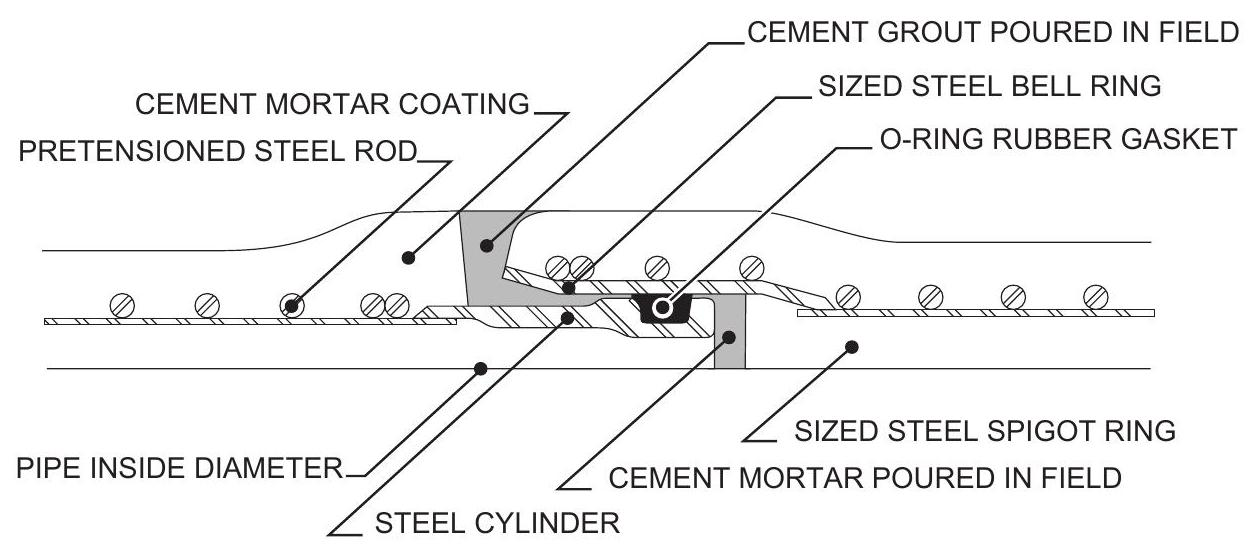
\includegraphics[max width=\textwidth]{PretensionedConcretePipe}

Pretensioned concrete cylinder pipe cross section

This pipe is connected by bell and spigot rubber ring push-on joints. Once the joint has been connected, the exposed steel must be coated with concrete to protect the steel cylinder from corrosion.

\section{High-Density Polyethylene (HDPE) Pipe}
High-Density Polyethylene (HDPE) is manufactured using a heat extrusion process and polyethylene resins. The material is used for water services lines and main lines. There are a wide variety of HDPE piping materials manufactured. The primary material used for drinking water is manufactured to meet ASTM standards D1248 and AWWA C-906. The designation used to identify the resin used to produce this piping material is ASTM, and the PPI (Plastic Pipe Institute) designation is PE 3408.

HDPE, PE 3408 is manufactured in pressure ratings from 65 psi to 220 psi. The most common material used in Alaska has a pressure rating of 160 psi. HDPE pipe is available in sizes of $3 / 4$ inch through 16 inches. Sizes of $3 / 4$ inch through $1.5$ inches are available in rolls of up to 500 feet, and a two-inch size is available in 350 -foot coils. Larger sizes, three inches and up, are available in 20 -foot and 40-foot lengths. All material used for drinking water is manufactured to IPS (Iron Pipe Size) outside dimensions. The wall thickness of the pipe increases with an increase in pipe diameter. The wall thickness is selected to maintain a ratio of pipe OD divided by wall thickness of 11 . This is called the SDR (Standard Dimension Ratio).\\

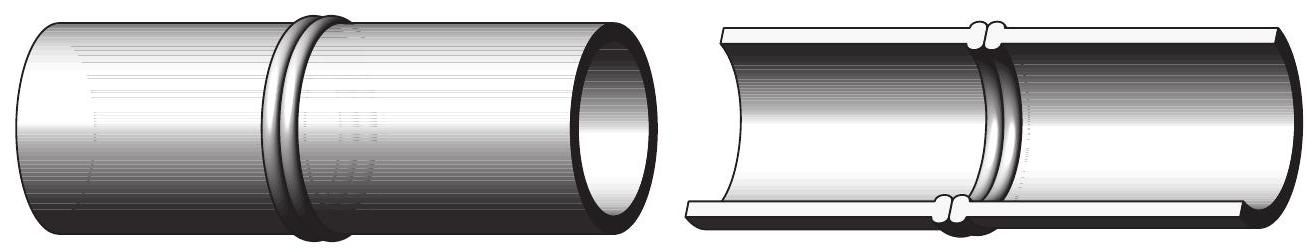
\includegraphics[max width=\textwidth]{HDPEFuseWeldJoint}

HDPE heat fused welded joint

The most common connection for HDPE pipe is a heat-fused weld. The pipe is commonly connected using a butt welding process. The welding of HDPE takes special equipment and special training. Small diameter (less than two inches) can be connected using compression fittings and stainless steel or brass insert fittings. There are special stainless steel adapters that allow the pipe to be connected using the Victaulic type of coupling. Flanged connections can be made by welding a butt or socket weld flange to the pipe. Repairs can be made to the pipe using typical cast iron couplings, provided that a special stainless steel insert is placed in the pipe to prevent collapsing of the pipe.

\section{Wood Pipe}
Wood pipe was at one time used quite extensively in the Pacific Northwest. For the most part, it has been replaced with one of the more common pipe materials previously described.

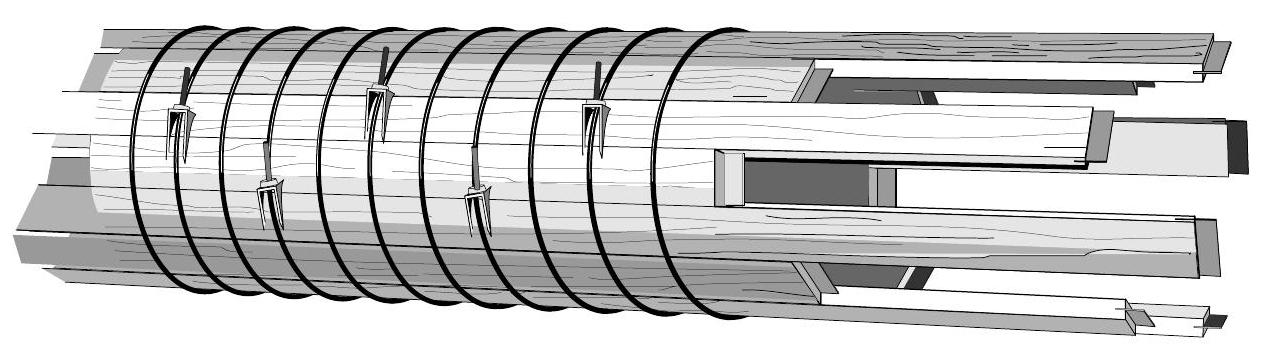
\includegraphics[max width=\textwidth]{2022_11_03_fc0cbc2f3612fab6edd2g-09(1)}

\section{Purple Pipe}
Continuous stave wood pipe

A special purpose for pipelines may be the distribution of reclaimed water. It is becoming more and more common for utilities to treat their wastewater to a high standard so that it can be reused for irrigation of athletic fields and golf courses, snowmaking at ski slopes, wetland enhancement, and commercial or industrial process water. Distribution pipe used to transport reclaimed water is either tinted or painted purple to distinguish it from potable water lines.

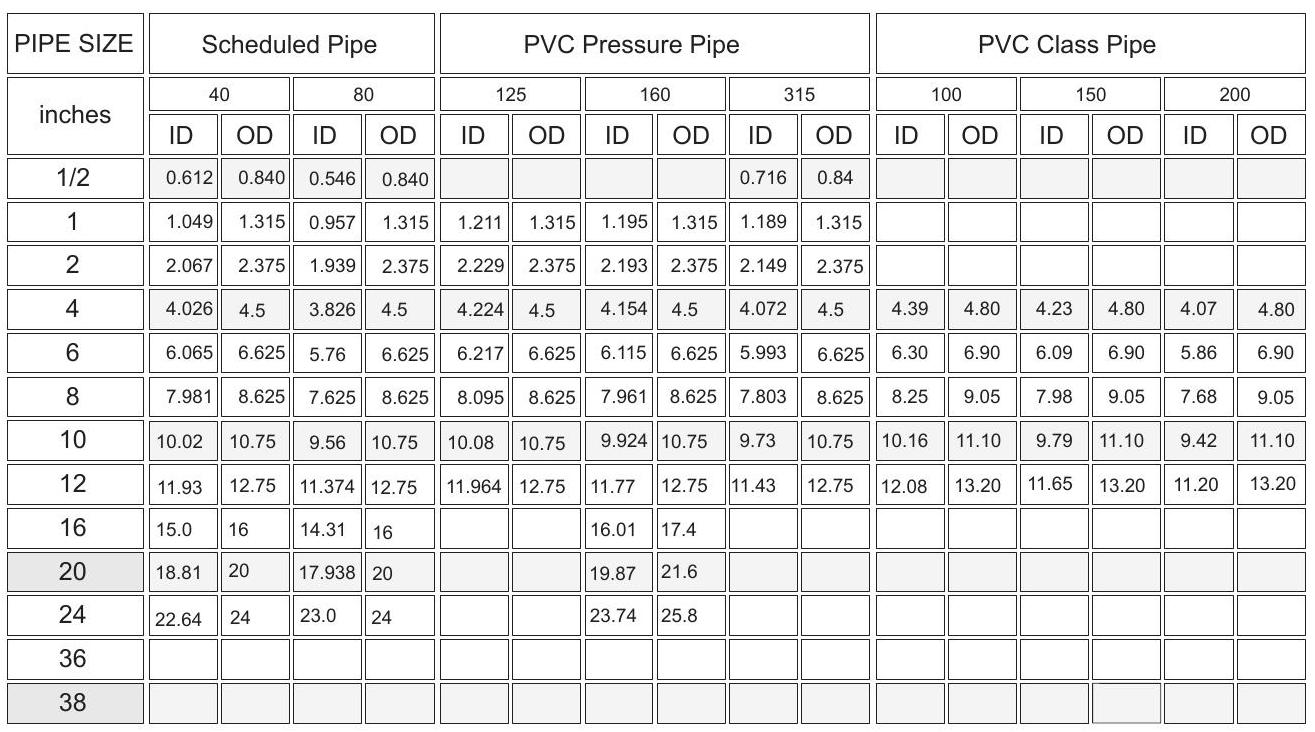
\includegraphics[max width=\textwidth]{2022_11_03_fc0cbc2f3612fab6edd2g-10}

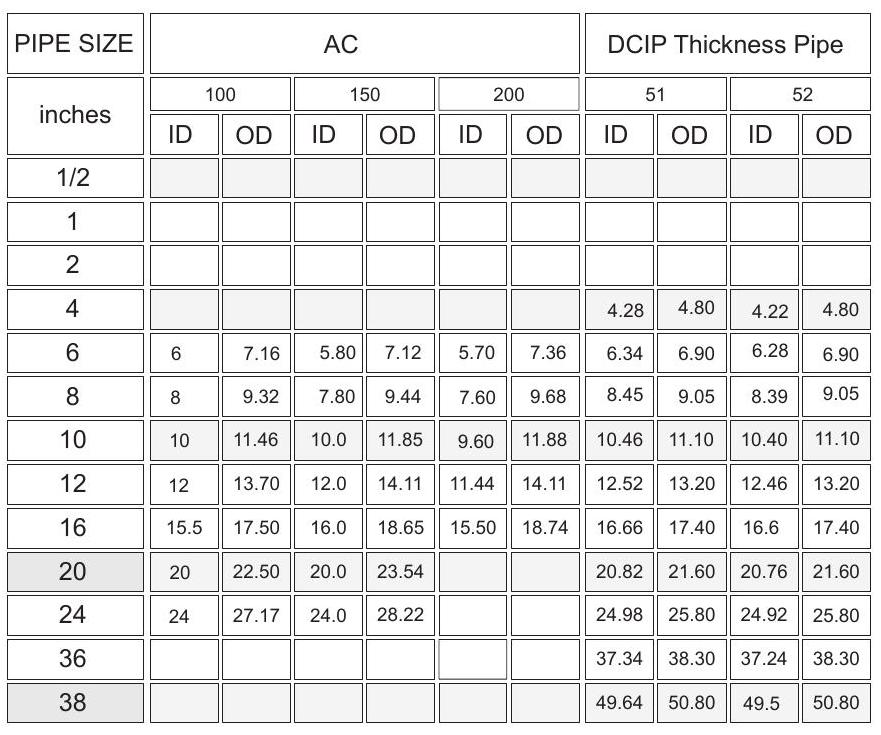
\includegraphics[max width=\textwidth]{2022_11_03_fc0cbc2f3612fab6edd2g-10(1)}

Inside and outside dimensions for common piping materials

${ }^{8}$ Appurtenances - Portions of a main structure necessary to allow it to operate as intended, but not considered part of the main structure: hydrants, valves, tees, elbows, etc.

\section{Fittings}
Fittings are used to connect other appurtenances ${ }^{8}$ and change the direction or size of the waterline. Some of the more common fittings are tees, wyes, bends, crosses, adapters, reducers, and increasers.

Fittings used in water distribution systems are made out of cast iron, PVC, HDPE, stainless steel, and fiberglass. The material selected is based on the piping material and local conditions.

The connections on cast iron fittings can be flanged, mechanical joint, or hub (with a rubber ring). Cast iron fittings are also available with combinations of any two connections. For instance, it is possible to obtain a cast iron fitting that is mechanical joint on one end and hub on the other end. Cast Iron fittings are typically used with PVC, AC, DCIP, and wood pipe.

Connections for steel fittings can be threaded, hub, flange, butt, or socket welded. Steel fittings are used with steel pipe. Stainless steel fittings can be threaded, hub, flange, butt, and socket welded. Stainless steel fittings are used with PVC and stainless steel pipe.

PVC fittings are made for PVC pipe and are either glued or hub. PVC pipe can be joined with tees, elbows, or other fittings manufactured for ductile iron pipe. HDPE fittings are made for HDPE pipe and are either socket welded or butt welded.

\section{Review}
\begin{enumerate}
  \item What type of hose should be used on haul trucks and watering points?

  \item What are two common piping materials used in distribution systems?

  \item What are the two most common DCIP joints?

  \item What is the standard length for four-inch diameter HDPE pipe?

  \item How is HDPE pipe connected?

  \item What type of piping material can be connected using a glue technique?

\end{enumerate}
\section{Pipe Installation}
\section{Distribution System Layout}
Water distribution mains may be laid out in grids, loops, or branches much like a tree. Grid or loop systems provide greater flow for fire protection and reduce the number of dead-end lines. Branch layouts result in a number of dead-end lines that can lead to bacteriological, taste, and odor problems. In addition, they require more frequent flushing and thus waste water.

Depressurization of a water line can lead to contamination if the surrounding soil is saturated with sewage or other groundwater contaminants. Water mains installed parallel to sewer mains must be at least 10 feet apart horizontally, and the water main must be one foot higher than any nearby sewer line. Water mains should never be laid in the same trench with sewer lines. In addition, water mains should be installed at least 25 feet horizontally from wastewater soil absorption systems (leach fields), cesspools, seepage pits, and septic tanks. In all situations, the location of water mains must meet the standards of the Alaska Department of Environmental Conservation and local or regional health agencies if applicable.

Prior to excavating, operators must determine the location of all buried water, sewer, electrical, gas, telephone, cable, and storm drain lines. The Alaska Digline is a onenumber, centralized call center established to provide information regarding underground utilities: 1-800-478-3121 or 1-907-278-3121. Alaska Digline agents use a database to pinpoint a reported area of activity and then send a standardized information packet to subscribers within two working days. ${ }^{9}$ Thrust Block - A concrete wedge placed between a fitting and the trench wall, used to transfer the force from the fitting to the trench wall, and thus prevent the fitting from being pushed away from the pipe. Whenever excavation is necessary for repairs or new construction, shoring may be needed to protect operators. A framework of metal and/or wood is placed in the trench to prevent a cave-in. Shoring components may consist of the following:

\begin{itemize}
  \item Sheathing

  \item Upright braces

  \item Horizontal jacks or cross braces

  \item Longitudinal braces or stringers

\end{itemize}
Often, a prefabricated aluminum trench box is used. The Alaska Department of Labor has specific safety rules regarding shoring that are discussed in another chapter of this manual.

Bedding is a granular material placed in the bottom of a pipe trench to support the pipe. A lack of proper uniform support can lead to "beam" breakage of the pipe.

Types of bedding include pea gravel, sand, and select native soil material. If a trench encounters bedrock, it must be over-excavated six inches before bedding is used to bring the trench up to the desired gradeline of the pipe. If the proper soil is available, some types of pipe, such as ductile iron, may be laid directly on the trench bottom. It is important to have an even pipe bedding and backfill over the pipe with soil that will not abrade the pipe walls. The backfill material must be adequately compacted with material that has sufficient moisture content.

Thrust forces are created in a pipeline where it changes direction, changes size, or dead-ends or at valve and hydrant locations. To prevent pipe joints from uncoupling and other damage from internal pressure or water hammer, a thrust block ${ }^{9}$ may be used. Thrust blocks are often made of concrete and steel reinforcement rods cast in place or large precast concrete blocks. It is important that thrust blocks rest against undisturbed soil with sufficient bearing area. There are standard engineering formulas to determine the thrust exerted within a pipeline and the size of thrust block necessary for a given type of soil.\\

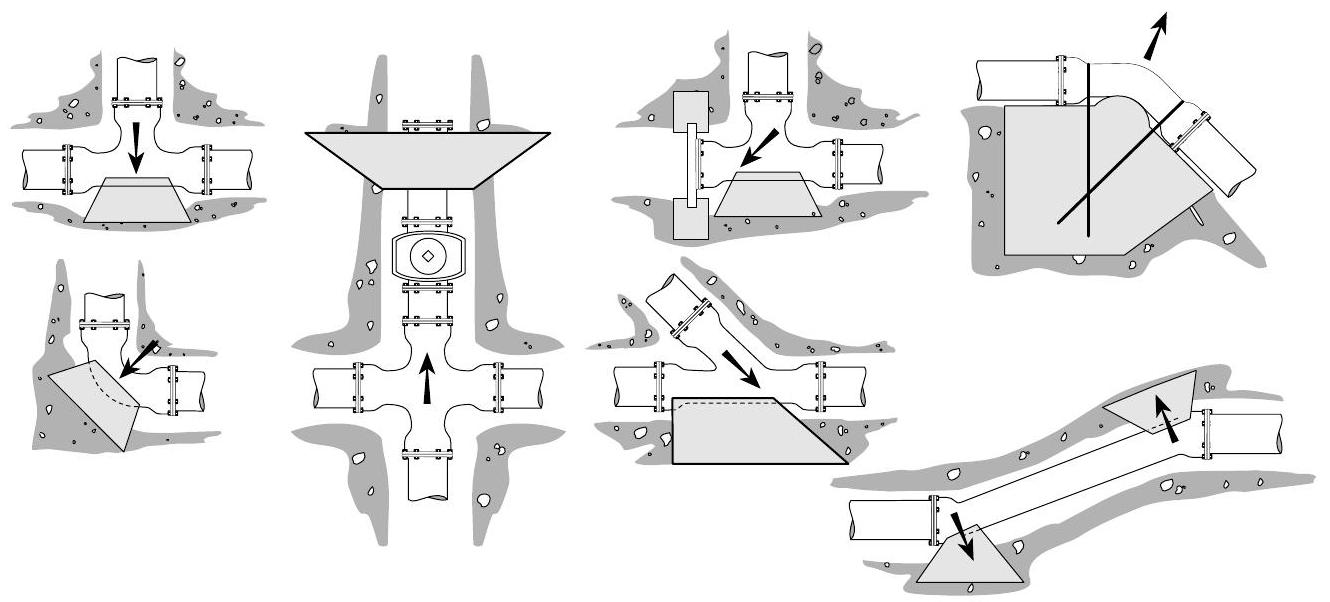
\includegraphics[max width=\textwidth]{ThrustBlocks}

Thrust blocks

Restrained joint fittings and short pieces of pipes called spools are designed to allow the connection of fire hydrants and branch valves to a distribution line without using a thrust block.

The most common restraining joints use a mechanical joint with some type of restraining device. One of these utilizes a snap ring placed into ductile cast iron or PVC pipe. The M.J. follower is machined to fit over the snap ring and hold the pipe and fitting in place. There are also a wide variety of proprietary fittings using various types of locking devices.\\

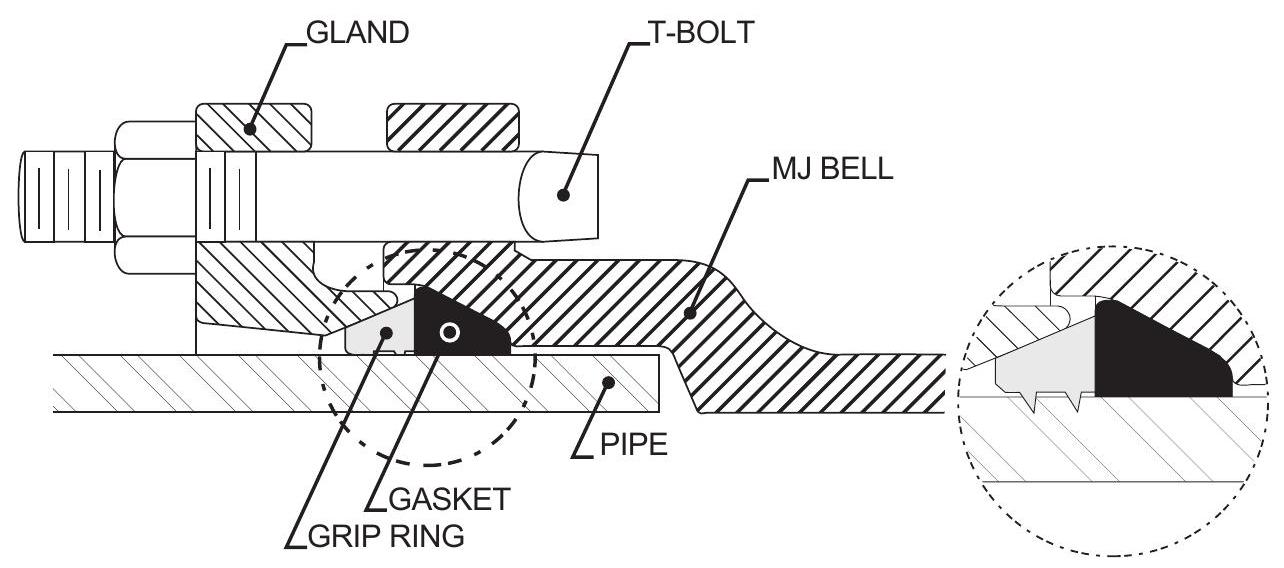
\includegraphics[max width=\textwidth]{2022_11_03_fc0cbc2f3612fab6edd2g-13}

\section{Pressure Testing and Disinfection}
Water should be delivered to the consumer at a minimum pressure of $35 \mathrm{psi}$ measured at the property line or meter. A typical working pressure in most systems is 60 psi. The absolute minimum pressure at all points in the distribution system is $20 \mathrm{psi}$, while $100 \mathrm{psi}$ is the maximum pressure desirable. Excess pressure will potentially damage water heaters, fixtures, and appliances.

Whenever a new pipeline is put into place and often after repairs are made, a leakage test is conducted. A valved-off section of the main line is slowly filled with water as air is expelled through a corporation stop or hydrant. After sitting idle for 24 hours, the pipe is brought up to a pressure 50 percent higher than the normal working pressure for the line, or $150 \mathrm{psi}$, whichever is larger. This pressure is maintained for four hours, after which pressure is observed for a drop that would indicate leakage.

The amount of water needed to refill the pipe is measured and compared to an allowable leakage rate calculated based on size and type of pipe. Leaks determined using this method along with any visible leaks are then repaired or replaced before the pipe is disinfected and flushed. Typically a hypochlorite solution of 25 to $50 \mathrm{mg} / \mathrm{L}$ is introduced into the pipe and allowed to sit for 24 hours prior to flushing. If calcium hypochlorite tablets are used for disinfection, the minimum contact time is 24 hours. The American Water Works Association (AWWA) has developed standards for conducting leakage/pressure testing and disinfection of water mains.

\section{Valves}
\section{Valve Types}
The types of valves used in distribution systems include gate, butterfly, globe, plug, ball, air control, vacuum breakers, check valves assemblies, and reduced pressure zone backflow prevention assemblies.

Check valves are used to prevent water from reversing direction in a line or flowing in two directions. The most common check valve used is the swing check, which has a simple design with a cast iron body and bonnet, a brass seat ring, and a movable disc. Flow forces the valve open, and when the flow is reversed, the flow closes the valve. Check valves are not adequate to control backflow or backsiphonage.

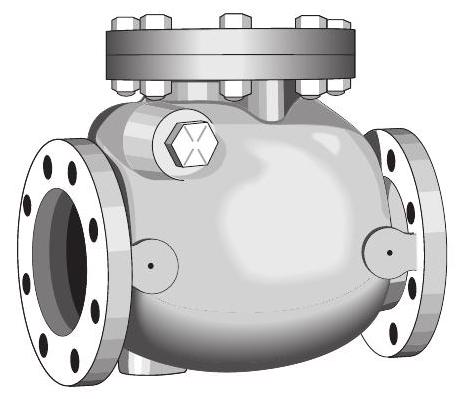
\includegraphics[max width=\textwidth]{SwingCheckValve}

Swing check valve

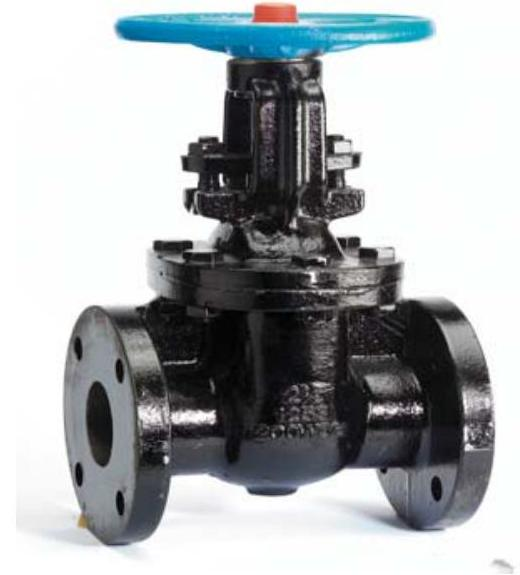
\includegraphics[max width=\textwidth]{GateValve}

Gate valve

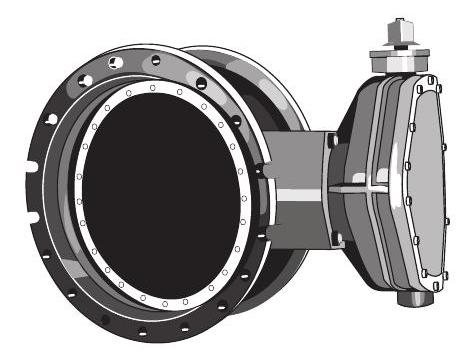
\includegraphics[max width=\textwidth]{ButterflyValve}

Butterfly valve

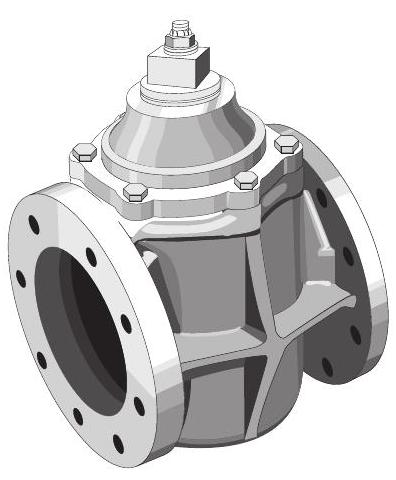
\includegraphics[max width=\textwidth]{PlugValve}

Plug valve ${ }^{10}$ Reservoir - A tank used to hold water.

" Backsiphonage - A form of backflow caused by a negative or belowatmospheric pressure within the water system.

\section{Function of Valves}
Valves are used in a water system to control pressure, control flow, regulate levels in reservoirs $^{10}$, isolate sections of line, release air, prevent vacuum in a distribution line, and prevent backflow and backsiphonage ${ }^{11}$. Globe valves are commonly used to regulate flow and pressure. Ball and plug valves are found in service lines. Both butterfly and gate valves are used in the main lines and hydrant lead lines in the distribution system. When butterfly or gate valves are used for isolation, they should be located at every intersection and intervals of not more than 800 feet so that small sections of the water main may be shut down for maintenance.

\section{Connections}
Connections on valves two inches and smaller are typically threaded, glued, or soldered, depending on the type of pipe. For larger valves, flange, mechanical joint, and hub are the most common connections. Valves can be purchased with a combination of connections. For instance, a mechanical joint by flange connection is fairly common.

\section{Gate Valves}
The lower portion of the gate valve, called the body, houses the connections and the seat that the movable closure comes up against. The closure is moved up and down by an operating stem. When in an open position, the closure is stored in the bonnet of the valve. The bonnet also holds the stuffing box, and the stuffing box contains the packing or "O" ring, which controls leakage around the stem. The common movable closures are single disc, double disc, and resilient seat:

\begin{itemize}
  \item Single disc - The single disc closure is wedge-shaped. When the valve is closed, the disc is forced down and against the seats on either side. This type of valve works only on low-pressure systems. When high pressure is applied to one side of the valve, it becomes very difficult to open.

  \item Double disc - The common movable closure used in the waterworks field is the double disc. The two discs are parallel to each other as are the two seats. When this valve is closed, a wedge of some type that rests between the two discs forces the two valve faces outward toward the two seats. When this valve is opened, the turning of the shaft causes the wedge to be relaxed and the two discs to move away from the seats, thus making it much easier to open the valve.

  \item Resilient seat - A recent addition to the gate valve market is a resilient seat valve. This valve uses a movable closure coated with a rubber-like material. The resiliency of the material allows for the use of a wedge-shaped single disc closure. Because of the resilient nature of the closure, the valve opens easily under high pressure.

\end{itemize}
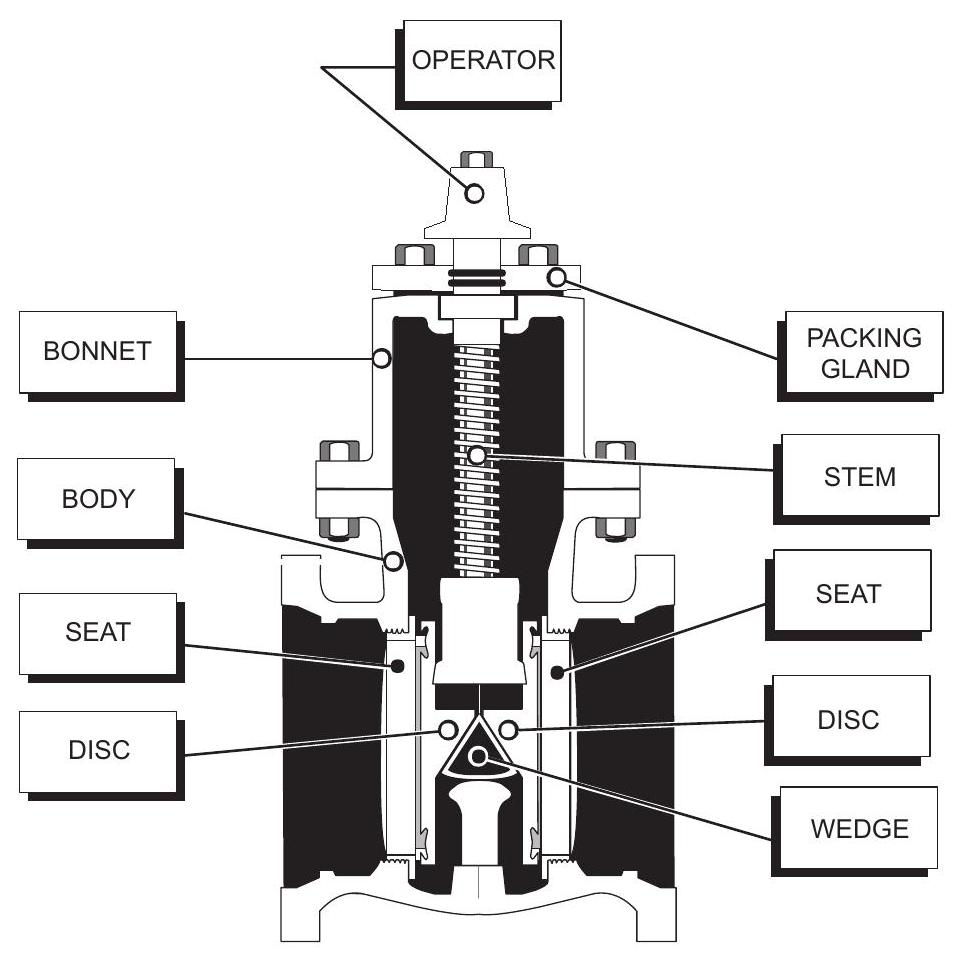
\includegraphics[max width=\textwidth]{GateValveDoubleDiskInside}

Cutaway of gate valve double disc

The stem found on a gate valve may either be rising or non-rising. Non-rising stems are used in most underground installations. In this valve, the disc moves up the stem, and only the stem rotates in the bonnet.

Rising stem gate valves are also called outside stem \& yoke (OS \& Y) gate valve. These are used in valve pits and on either side of control valves. They allow easy determination of whether the valve is open or closed.

The device used to turn the stem is called a valve operator. Common operators are two-inch square nuts on underground installations and hand wheels on valve pit installations. ${ }^{12}$ Butterfly Valve $-\mathrm{A}$ valve whose movable closure rotates $90^{\circ}$ around a shaft that is set through the center of the closure and the center of the flow path.

\section{Butterfly Valves}
The butterfly valve ${ }^{12}$ has a movable closure that rotates on a shaft inside of the valve body. The body holds the inlet connections and valve seat. When closed, the movable closure seats against a rubber-like seat that is set into the valve body or fastened to the closure. The butterfly valve is not 100 percent watertight when closed.

The valve stem usually passes into a gear train. The common gear train is a $90^{\circ}$ gear train, which allows the valve to be mounted sideways. When installed in the ground, the operator is commonly a two-inch square nut. A wheel is used when the valve is installed in an open valve pit.

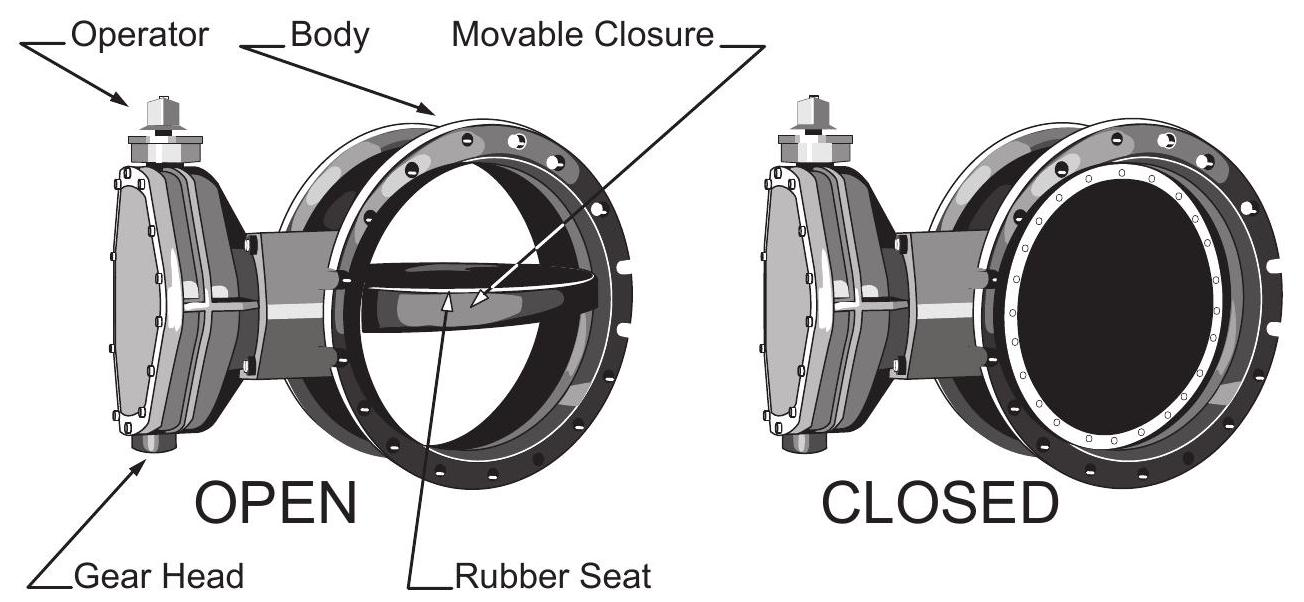
\includegraphics[max width=\textwidth]{ButterflyValveOperation}

Butterfly valve operation

Butterfly valves offer some restriction to flow, which increases headloss. They are, however, much easier to open and close in large lines than gate valves.

\section{Air Valves}
There are three common air valves used in a distribution system: air vacuum, air relief (release) and combination valves. Each valve has its own unique function:

\begin{itemize}
  \item Air and vacuum valves - Air and vacuum valves are designed to allow the escape of air while the line is being filled. Once the line is filled, the pressure in the valve keeps the valve from opening even if air accumulates in the valve. When the line is drained and the internal pressure drops below atmospheric, the valve opens, allowing air in preventing the pipe from collapsing. These valves are also referred to as air relief valves.

  \item Air relief valves - Air release valves are commonly installed at high points in a system and are designed to collect and release air that accumulates in the system. An accumulation of air in a pipe will reduce its flow capacity. Another application of an air relief valve is to vent air that has accumulated in the well column when a well was not in use.

  \item Combination valves - There are two types of combination valves. The most common is the combination of air release and vacuum relief, a combination of the two valves described above and shown in the diagram below. This type of valve is often referred to simply as an air vac valve. The second combination valve is one designed with two orifices, one for high airflow and one for low airflow. This is a combination air relief valve. Combination air vac valves are installed at high points in the line to allow air in and out of the line. Allowing air out of the line reduces problems with low flows due to a blockage by air. Allowing air into the line during times when the line may be being emptied prevents the low internal pressure from drawing a joint gasket into the pipe and thus causing a leak.\\

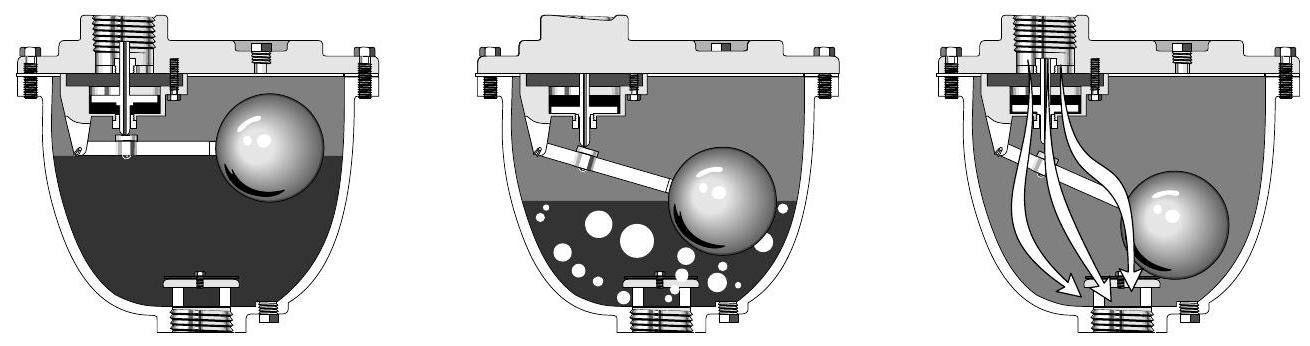
\includegraphics[max width=\textwidth]{AirVacuumValve}

\end{itemize}
Combination air vacuum valve

Air vac valves are installed on top of the line usually through a two-inch corp stop with a two-inch gate valve placed between the corp stop and the valve. The entire setup is normally placed in a valve pit.

\section{Globe Valves}
The globe valve is used to reduce or control pressure in a portion of a system, to throttle or control flow from a pump, to reduce water hammer ${ }^{13}$ at a pump, and to control the level of water in a reservoir. When a valve is used to control the level of water in a reservoir, it is called an altitude valve ${ }^{14}$. A specialized globe valve used to dampen water hammer is a pressure-relief valve.

Globe valves have a movable closure that moves up and down inside of the valve body. The movable closure is usually attached to a shaft that is positioned by two guides. The movable closure either seats against a resilient face, or the closure has a resilient face that seats against a solid valve seat. The position of the movable closure is controlled by pressure on a diaphragm or piston at the top of the valve. The diaphragm pressure is obtained directly or indirectly from the water system. The control of this pressure is usually regulated through a pilot valve. Most of the globe valves used for flow and pressure control and as altitude valves use flange connections on each side.

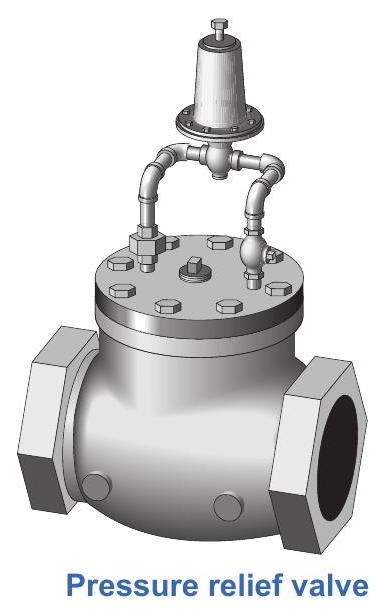
\includegraphics[max width=\textwidth]{PressureReliefValve}

\section{Plug Valves}
Plug valves can be found in a wide variety of sizes. In a water system, they are commonly used as the isolation valves on the customer service lines. In this instance, they are usually made of brass and have threaded or copper tubing connections.

The plug valve is the simplest of all valves. The movable closure has a hole through which water is permitted to pass. $\mathrm{A} 1 / 4$ turn turns the valve from open to closed.

Older plug valves control leakage between the movable closure and the valve body by the close tolerance between the two components. This close tolerance makes it difficult to open and close these valves. In recent years, plug valves have been manufactured with Teflon ${ }^{\mathrm{TM}}$ and "O" ring seals. These valves are much easier to operate. ${ }^{13}$ Water Hammer - The result of the conversion of velocity head to pressure head. The pressure spike created by suddenly stopping the flow of water. ${ }^{14}$ Altitude Valve $-\mathrm{A}$ valve that automatically opens and closes to maintain the level of water in a reservoir. Most commonly a wide body globe valve.\\

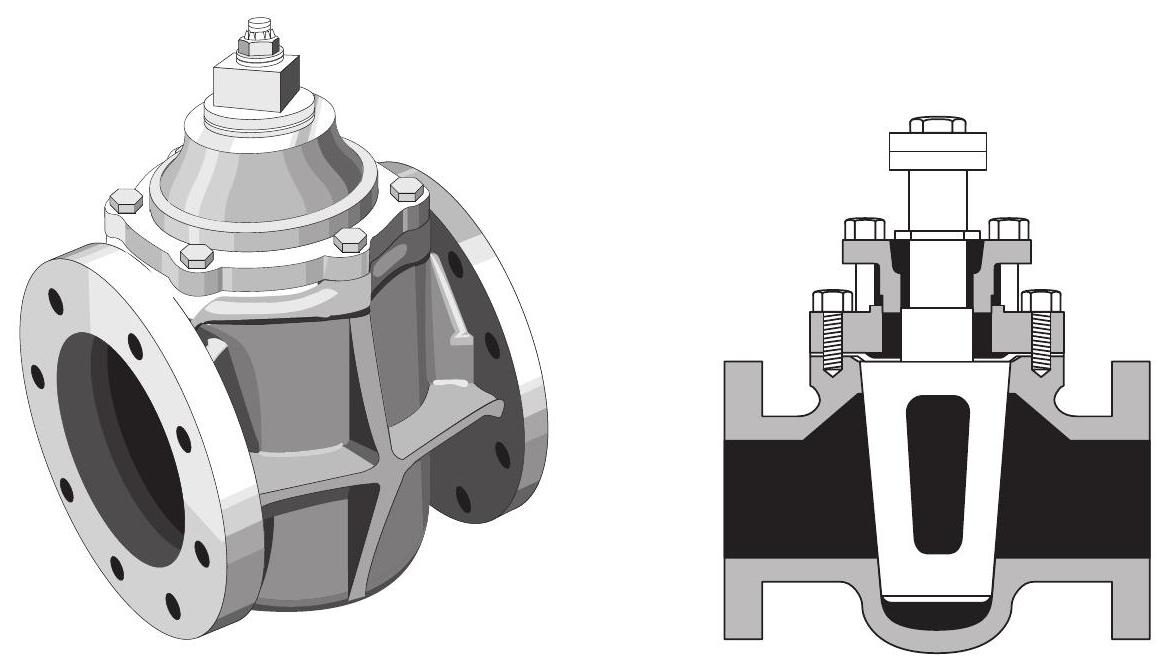
\includegraphics[max width=\textwidth]{PlugValve2}

Plug valve

\section{Ball Valves}
Ball valves are found on small lines (less than two inches), in and around the treatment plant, and on some customer service lines. They are manufactured from brass or PVC. They offer an advantage over the plug valve because they are much easier to operate. Large ball valves (greater than three inches) are used as flow and pressure control valves on pumping systems. These large ball valves are commonly manufactured from cast iron with a steel movable closure.

The ball valve is similar to the plug valve. The movable closure has a hole in its center through which water passes. Closing or opening the valve is accomplished by a simple $1 / 4$ turn of the handle. The ball valves movable closure is prevented from leaking by seals placed in the valve body.\\

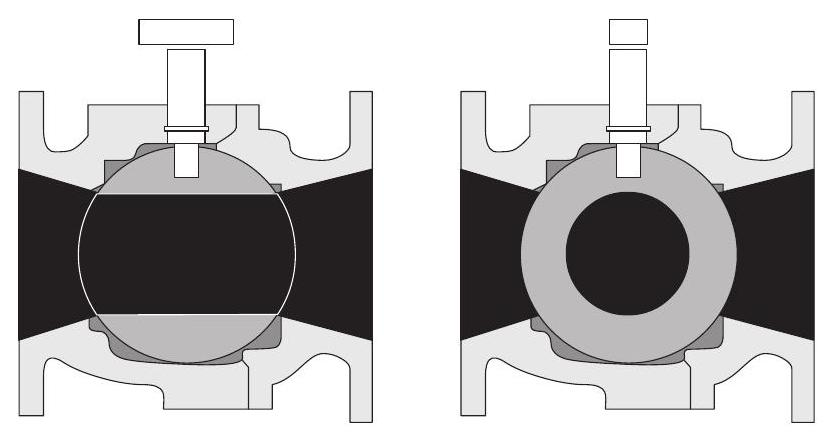
\includegraphics[max width=\textwidth]{BallValveInside}

Ball valve open and closed

A foot valve may be installed at the bottom of a well discharge line or the end of the intake pipe in a suction lift pumping situation. The function of this valve is to prevent the water column from discharging back into a well or wetwell and to maintain prime to the pump.

\section{Valve Boxes}
Access to main line valves on piped systems is through a valve box. Valve boxes are made of cast iron, concrete, or PVC with a cast iron lid.

\section{Valve Maintenance}
All valves in the main lines of the distribution system should be located and exercised once each year. This is best done in early summer to allow repair before winter.

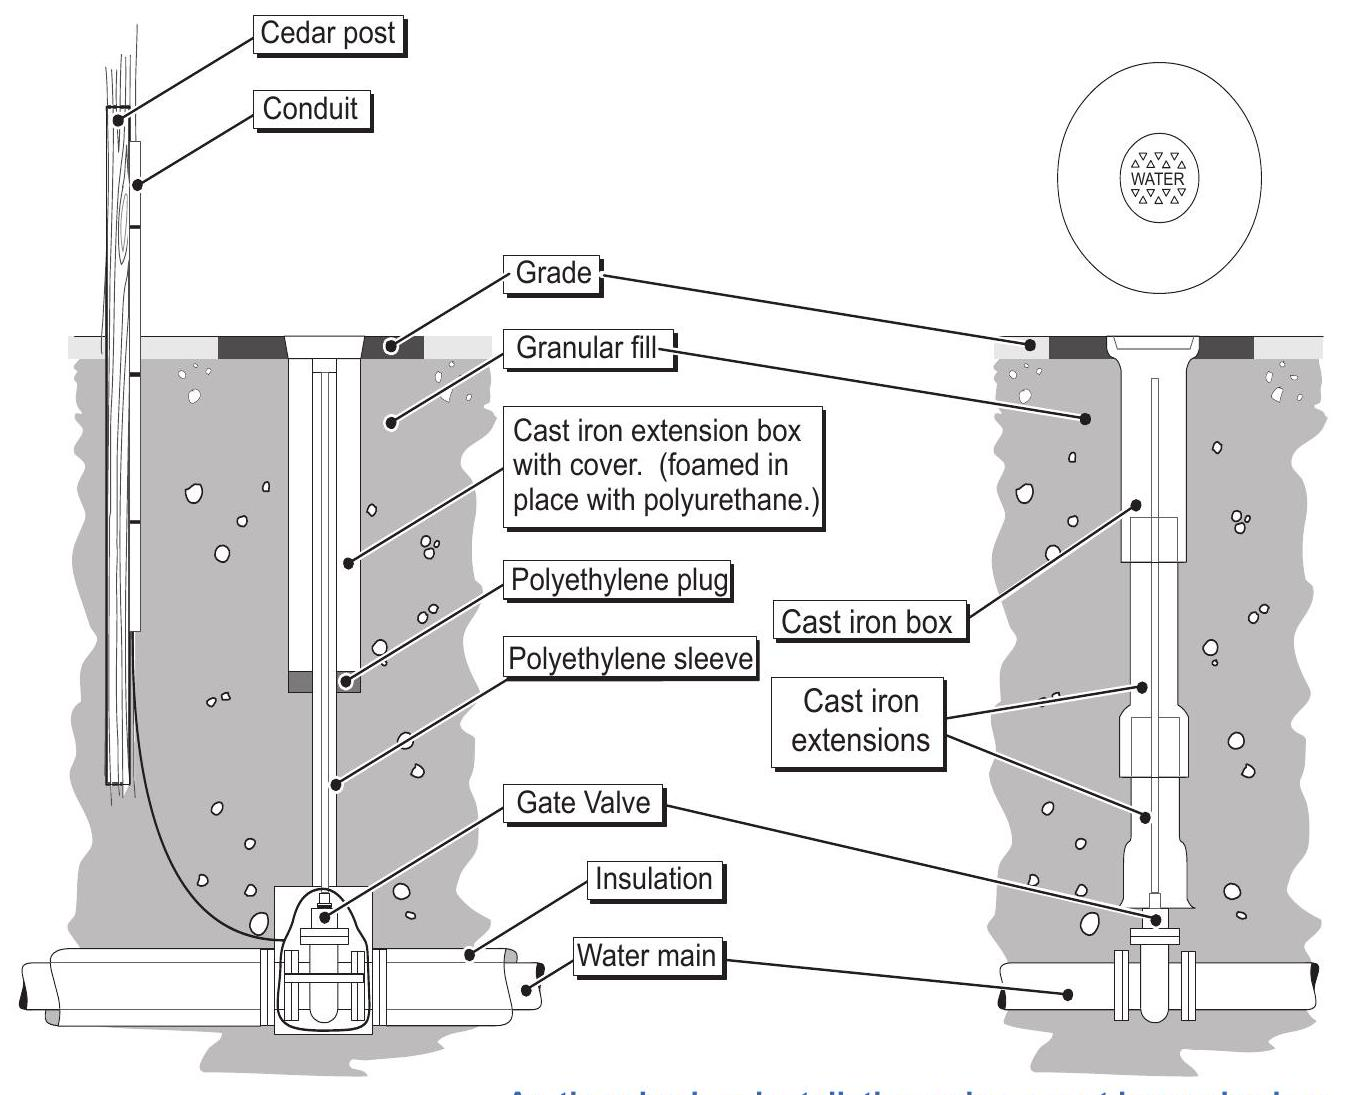
\includegraphics[max width=\textwidth]{2022_11_03_fc0cbc2f3612fab6edd2g-19}

Arctic valve box installation using a cast iron valve box

\section{Identification}
\begin{enumerate}
  \item Identify the valves below.
\end{enumerate}
\includegraphics[max width=\textwidth]{2022_11_03_fc0cbc2f3612fab6edd2g-20}

\begin{enumerate}
  \item 
\end{enumerate}
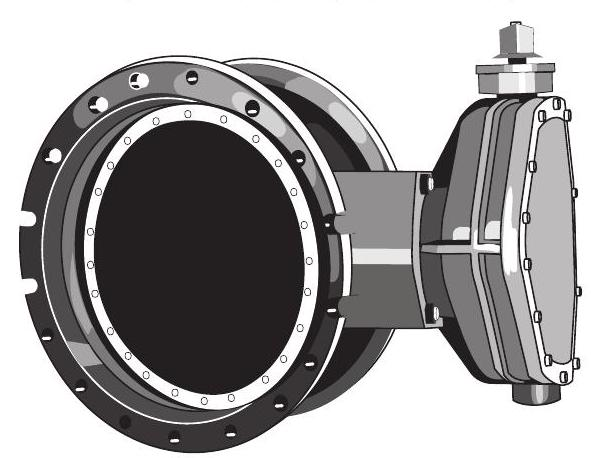
\includegraphics[max width=\textwidth]{2022_11_03_fc0cbc2f3612fab6edd2g-20(1)}

\begin{enumerate}
  \setcounter{enumi}{3}
  \item 
\end{enumerate}
\includegraphics[max width=\textwidth]{2022_11_03_fc0cbc2f3612fab6edd2g-20(2)}

\begin{enumerate}
  \setcounter{enumi}{2}
  \item 
\end{enumerate}
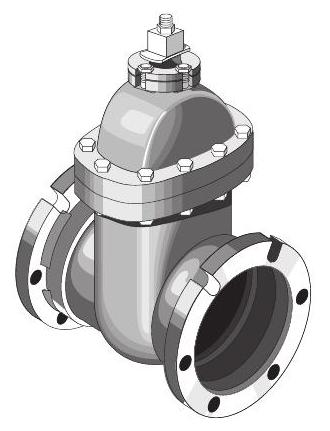
\includegraphics[max width=\textwidth]{2022_11_03_fc0cbc2f3612fab6edd2g-20(3)}

\begin{enumerate}
  \setcounter{enumi}{4}
  \item 
\end{enumerate}
\section{Identification}
\begin{enumerate}
  \item Identify the valve components below.

  \item 
  \item 
  \item 
  \item 
  \item 
  \item 
  \item 
\end{enumerate}
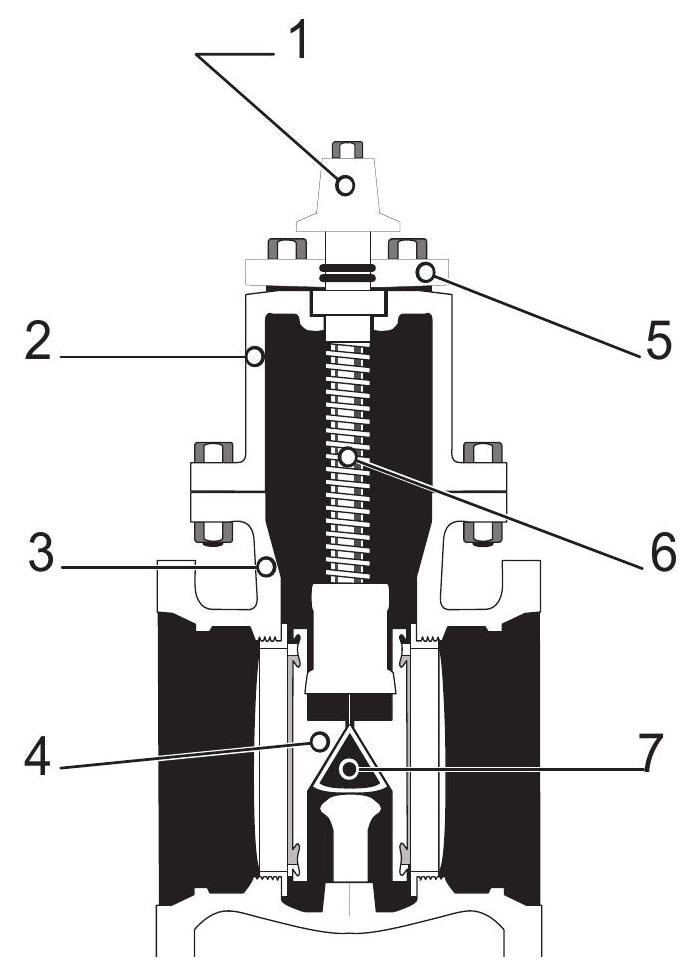
\includegraphics[max width=\textwidth]{2022_11_03_fc0cbc2f3612fab6edd2g-20(4)}

\section{Purpose}
\section{Fire Hydrants}
The primary function of a fire hydrant is to provide access to water for fire suppression. Fire hydrants can also be used in the following secondary functions:

\begin{itemize}
  \item Access to water for construction

  \item Access to water for other utilities, such as street cleaning and sewer cleaning

  \item Access point for testing the distribution system's flow capabilities

\end{itemize}
\section{Hydrant Types}
Two classifications of hydrants are made in the United States: the wet barrel and the dry barrel. These are manufactured in accordance with AWWA standards C-502 and C-503:

\begin{itemize}
  \item Wet barrel - Wet barrel hydrants have the operating valve in the nozzle section of the hydrant and are operated by rotating the operating stem on each of the outlets. These hydrants are used in warm climates where it rarely freezes. Their main advantage is the ease of connecting a second fire truck. Each discharge port is independently valved.

  \item Dry barrel - Dry barrel hydrants have the operating valve installed below ground. The hydrant is equipped with a special drain valve that allows the above ground portion to automatically drain when not in use. The dry barrel hydrant is widely used in colder climates. Its main advantage is that it is less likely to freeze, and when hit by a vehicle, it does not normally lose water.

\end{itemize}
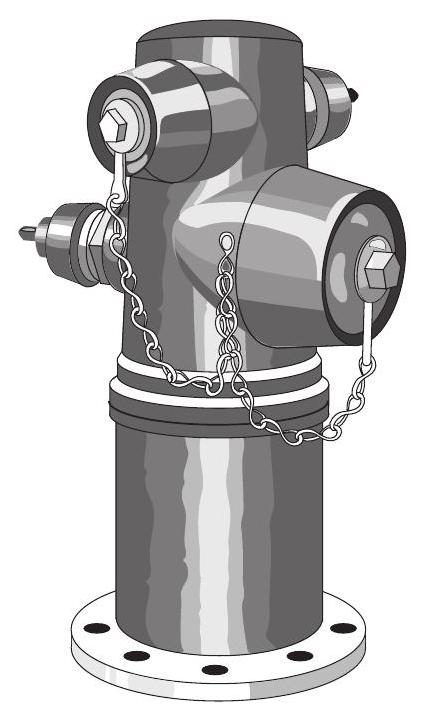
\includegraphics[max width=\textwidth]{WetBarrellFireHydrant}

Wet barrel fire hydrant

\section{Four Types of Dry Barrel}
Four types of dry barrel fire hydrants are used in the United States. Two of the types are called compression hydrants. There is one type of compression hydrant ${ }^{15}$ that opens with the flow, and one that opens against the flow. A third type of dry barrel hydrant is called the toggle hydrant ${ }^{16}$, and the fourth type is the slide gate hydrant ${ }^{17}$. All of these hydrants are opened by turning an operating nut on the top of the hydrant. On both of the compression hydrants, the main valve, which is made of a soft

\includegraphics[max width=\textwidth]{DrybarrellFireHydrant1}

${ }^{15}$ Compression Hydrant - A fire hydrant where the main valve moves reciprocally on a vertical axis is against a seat located in the hydrant base. The valve moves against the seat to close and away from the seat to open.

${ }^{16}$ Toggle Hydrant - A fire hydrant where the main valve moves reciprocally on a horizontal axis against or away from a vertical seat located in the base of the hydrant. The main valve is moved by means of a vertical stem. Rotation of the stem causes the arms of the toggle mechanism to move the main valve.

${ }^{17}$ Slide Gate Hydrant - A fire hydrant where the main valve moves vertically by means of a threaded stem. When the stem is rotated, the internally threaded gate moves. The gate is forced against the valve seat by a wedging mechanism. material, is moved up or down away from a bronze seat. The toggle hydrant uses a sideways action to move the valve against a bronze seat. The slide gate works more like a single disc gate valve. The gate is forced down by the stem and sideways against a seat by a wedge.

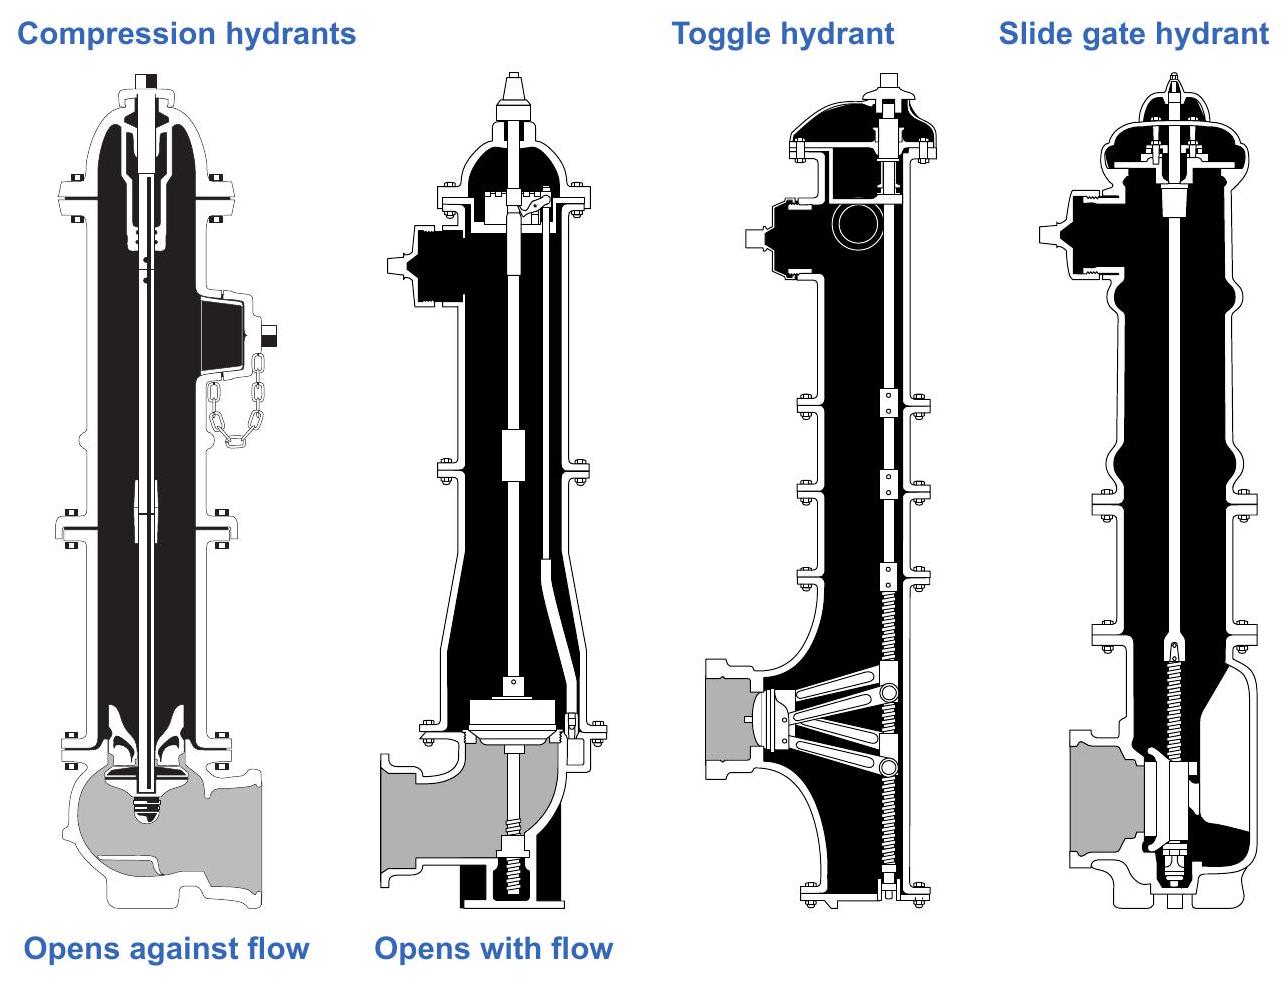
\includegraphics[max width=\textwidth]{OtherDryBarrellFireHydrant}

Hydrants are also classified by whether they are post or flush hydrants. The hydrant that we commonly think about is a post hydrant. A flush hydrant sits flush with the surface of the ground and is used in airports, on bridges, and other places where the exposure of the hydrants is more of a hazard than the difficulty of connecting to a ground-level hydrant.

For safety purposes, hydrants can also be designed to break at the ground line with a minimum amount of damage. This type of hydrant is referred to as a traffic model hydrant.

Special methods have been devised to allow access to above and below-ground utilidor systems. One such method uses an angle globe valve connected to the main line. While this does not meet the AWWA standards for a fire hydrant, it does function as a fire hydrant.\\

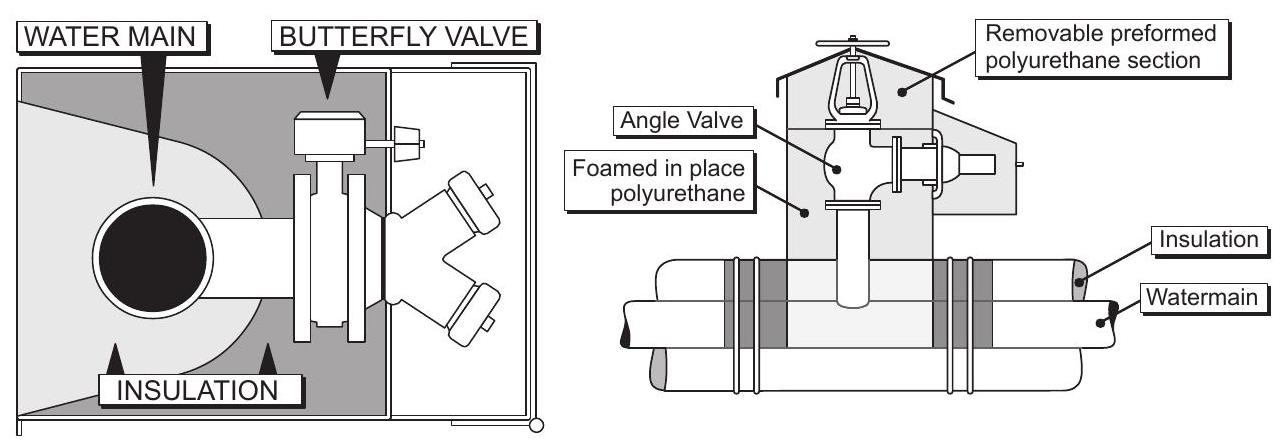
\includegraphics[max width=\textwidth]{2022_11_03_fc0cbc2f3612fab6edd2g-22(1)}

Arctic hydrants

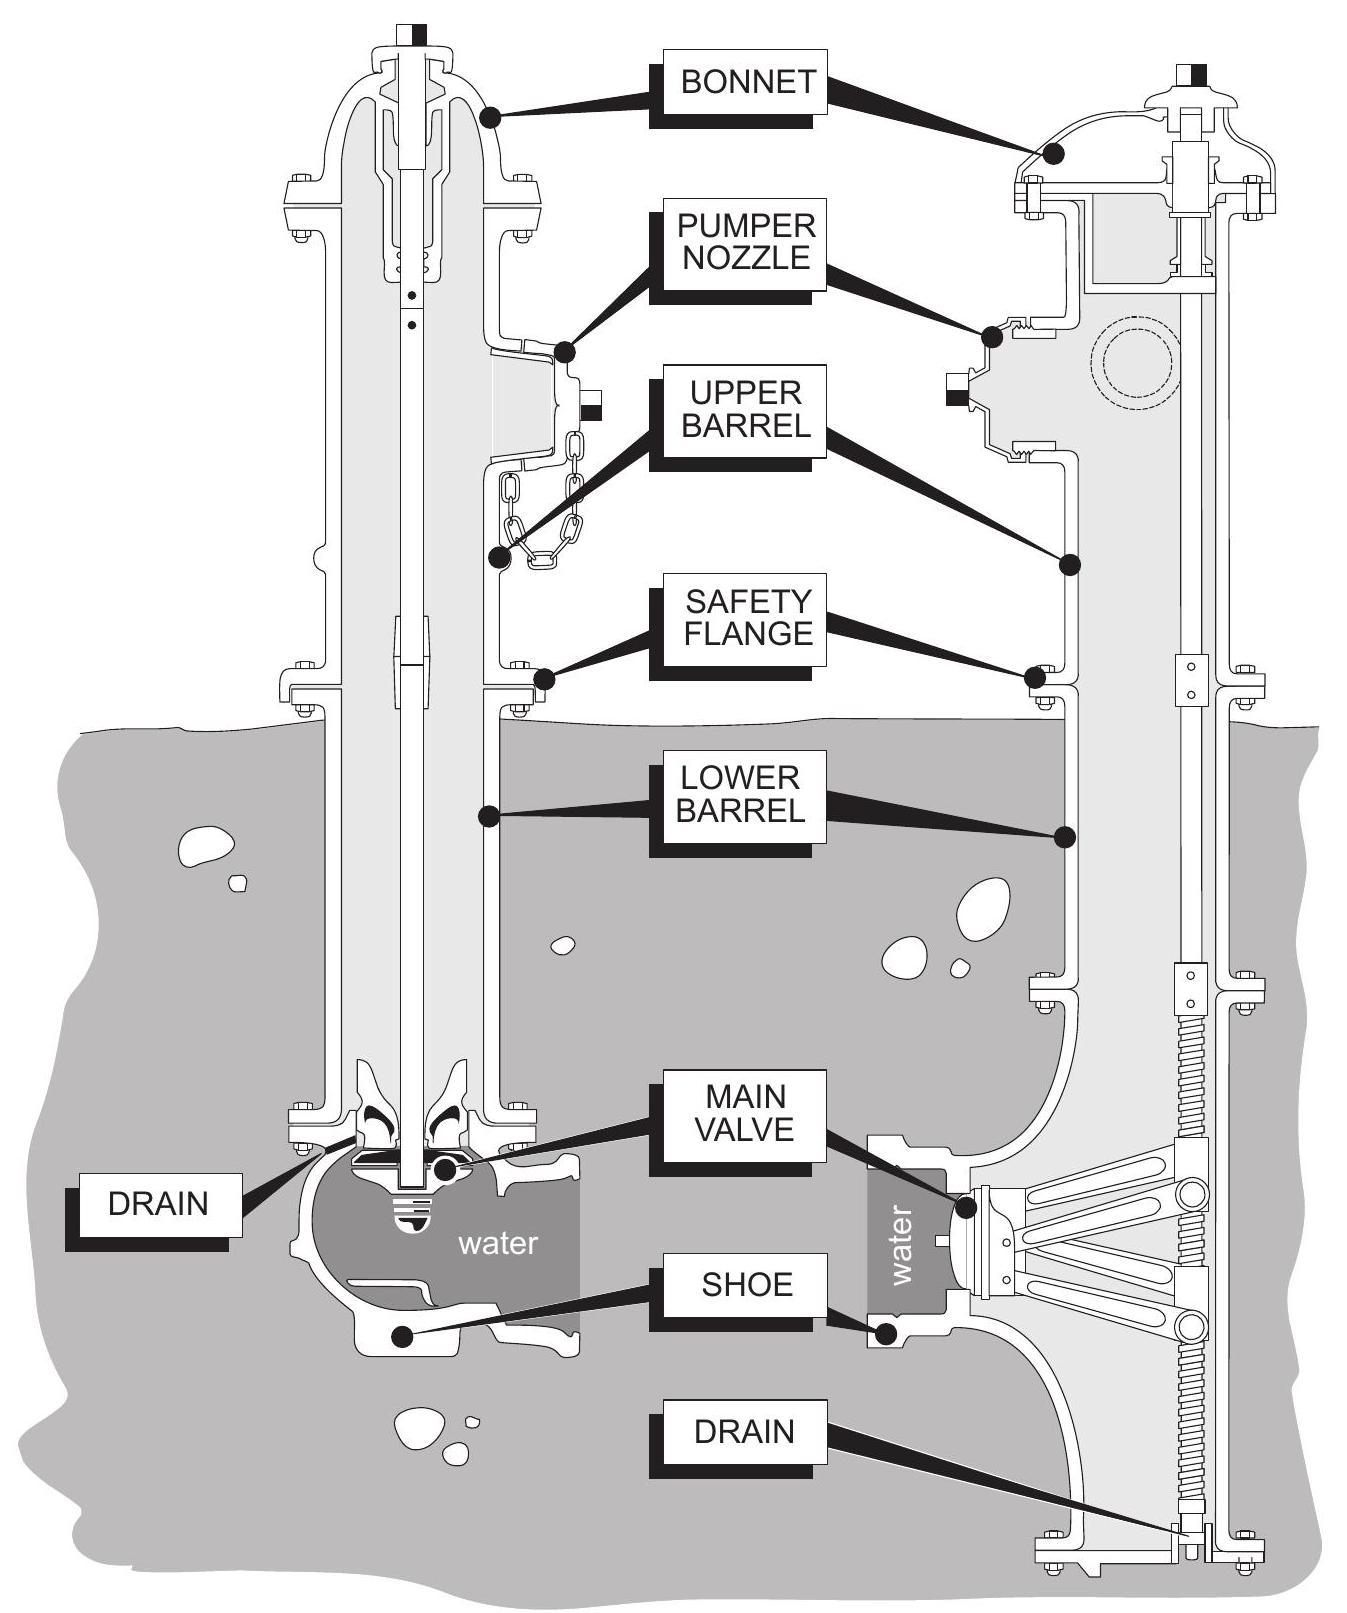
\includegraphics[max width=\textwidth]{2022_11_03_fc0cbc2f3612fab6edd2g-23}

\section{Hydrant Components}
If you examine the hydrant from the top down, the major components are identified as follows:

\begin{enumerate}
  \item Bonnet - On top of the upper barrel sits the bonnet. The bonnet protects the packing and the operating nut mechanism.

  \item Upper barrel - The upper barrel contains the outlet nozzles and a plate that holds packing or "O" rings, which prevent water from entering the top of the hydrant. Common nozzle configurations include two $21 / 2$-inch hose nozzles and one pumper nozzle that may be any size from four through six inches. Some hydrants do not have packing plates and are referred to as wet barrel hydrants.

  \item Lower barrel - The next section is the lower barrel. This section determines the height or bury ${ }^{18}$ of the hydrant. The bury is the distance from the bottom of the inlet connection (invert ${ }^{19}$ ) to a point four inches below the flange that connects the lower barrel to the upper barrel.

\end{enumerate}
${ }^{18}$ Hydrant Bury - The distance from the invert of the hydrant lead to a point four inches below the flange between the upper and lower barrels of a hydrant.

19 Invert - The bottom inside surface of a pipe. ${ }^{20}$ MVO (Main Valve Opening) - The inside diameter of the bronze main valve seat of a fire hydrant. 4. Shoe-The shoe is where the inlet connection is made. The inlet connection can be either a four- or six-inch M.J., hub, flange, or screwed connection. The shoe also changes the direction of the flow from horizontal to vertical. On most compression hydrants, the main valve is housed either in the shoe or directly on top of it. The size of the main valve is referred to as the main valve opening $\left(\mathbf{M V O}^{20}\right)$. This is the inside diameter of the valve seat. Sizes ranging from four through six inches are common. The shoe also usually contains the drain valve assembly, which is used to drain the hydrant when it is closed.

\section{Hydrant Maintenance}
Fire hydrants should be inspected for leakage and proper operation and exercised at least once each year. This is best done in early summer so that any necessary repairs can be made before winter.

\section{Customer Service Materials}
\section{Meters}
While not all communities install meters on customer services, meters serve at least two functions:

\begin{enumerate}
  \item They provide a method to fairly distribute the cost of providing water service.

  \item Having meters allows the operator to determine the amount of unaccountedfor water lost by the system. High percentages of unaccounted-for water indicates excessive leakage in the system.

\end{enumerate}
Customer services are divided into at least three categories: household, commercial, and fire. The type of meter used often depends upon the type of service.

\section{Household}
The standard meters for household services are $5 / 8$ inch to one inch in size and provide at least 20 to $30 \mathrm{gpm}$ at $40 \mathrm{psi}$. A household meter has a register that records the quantity of water used, a magnetic connection to a rotating device, a measuring chamber, a body, and, in some cases, a bottom plate that will break when frozen to prevent damage to the meter.

There are three types of household meters. They are described by their different measuring chambers. The nutating disk and oscillating piston meters are called displacement meters. With these meters, water causes a piston or disk to be moved, displacing the water and causing the rotating assembly to rotate, which indicates flow on the register. The turbine meter uses a vaned wheel that is rotated by the flow of water. The wheel is attached to the register, thus indicating water use.

Household meters are installed in meter boxes in the sidewalk in locations where the frost depth is only two or three feet. In locations where meters are apt to freeze each winter, they are installed in the house.

In Alaska's small communities, Badger, Rockwell, and Neptune are the most common brands of household meters used.

\section{Commercial}
Commercial services are usually considered any services serving something other than a single household and having a service line one inch or larger in size.

There are three common commercial meters:

\begin{itemize}
  \item Compound meters - The compound meter has two measuring chambers: one for low flow and one for high flow. The low flow chamber typically uses a displacement meter, while the high flow chamber uses a turbine or propeller meter.

  \item Turbine meters - Turbine meters typically use a pinwheel mounted on a vertical shaft. Turbine meters in large sizes have low accuracy.

  \item Propeller meters - Propeller meters use a prop blade mounted on a horizontal shaft in the flow. Propeller meters work best over a narrow flow range and are used on services where the flow does not vary widely.

\end{itemize}
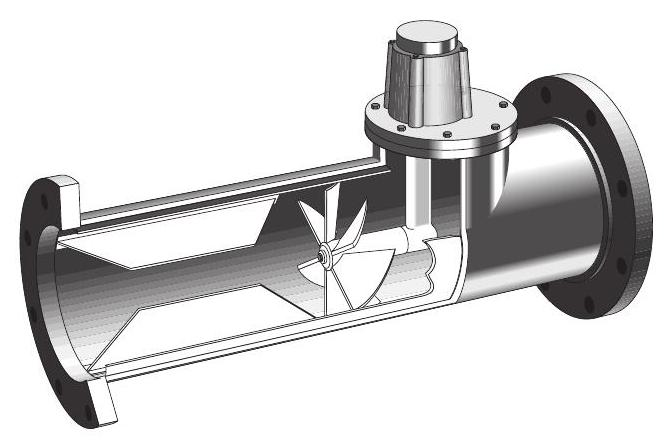
\includegraphics[max width=\textwidth]{TurbineMeter}

Turbine meter

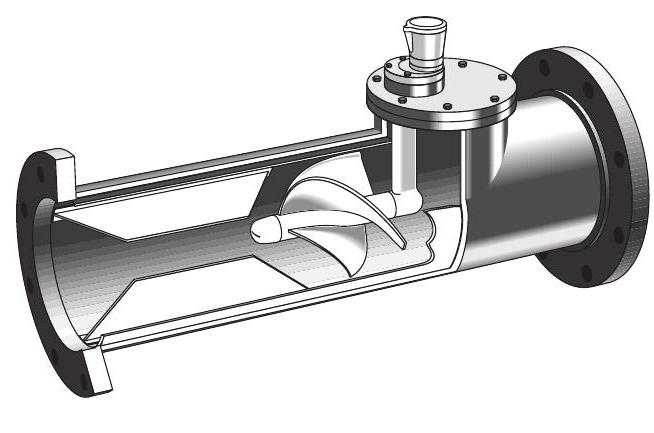
\includegraphics[max width=\textwidth]{PropellerMeter}

Propeller meter

\section{Fire}
Meters installed on fire sprinkler lines are called fire service meters or check meters. The most common contains a large swing check valve and a small displacement meter. When there is a fire, the check opens and a small amount of water is diverted through the small meter, indicating that there has been a flow in the line.

\section{Service Fittings}
Services can be connected to an existing main line without shutting the line off. This is done using a special tapping machine. The tapping machine allows direct connection to ductile cast iron pipe or connection to AC, PVC, and HDPE through a saddle, a malleable iron or brass device that is clamped around the line. A gasket prevents leakage between the saddle and the pipe.

Services are connected to the main line through a brass plug valve called a corporation stop. The corporation stop may be threaded into a tee, tapped directly into a cast iron pipe, or threaded into a saddle. The tapping machine can be connected to the corporation stop, and a drill bit can be used to tap the main.

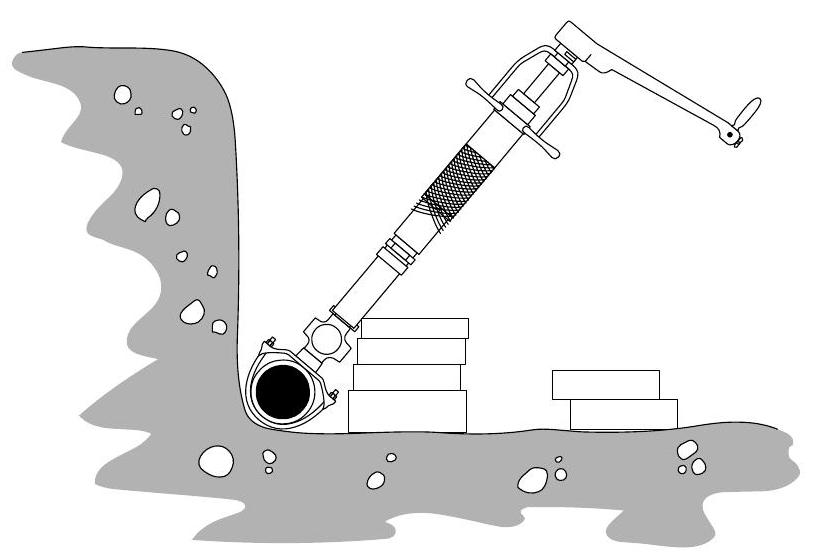
\includegraphics[max width=\textwidth]{2022_11_03_fc0cbc2f3612fab6edd2g-26}

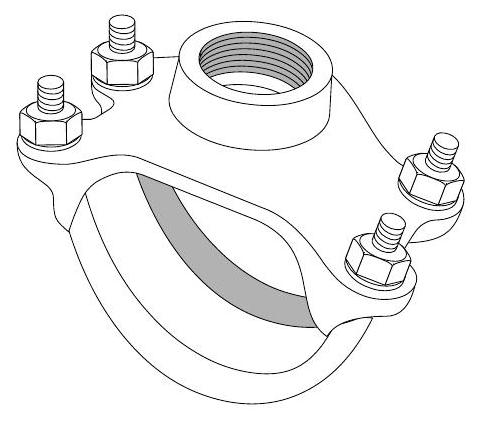
\includegraphics[max width=\textwidth]{ServiceSaddle}

Service saddle

Tapping machine

\section{Corporation stop}
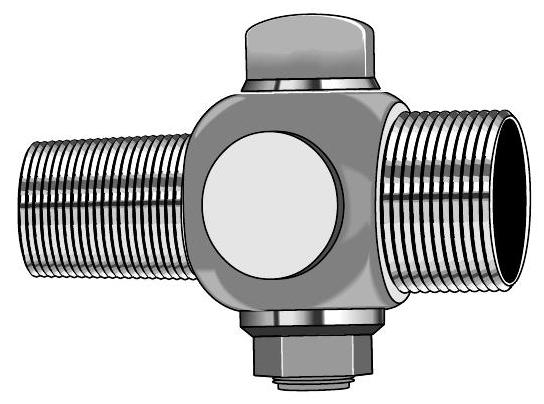
\includegraphics[max width=\textwidth]{CorporationStop}

When the meter is installed in the house or when there is no meter, the utility needs a way to shut off the service. This is accomplished with a brass plug valve called a curb stop. The curb stop is placed in the service line in a location that allows access through a curb stop valve box from outside the house. A connection to the curb stop is often the location of leaks in older service installations.

The brass valve that is fastened to the meter is called an angle stop or straight stop, depending upon its obvious shape. This valve is used to shut off the service.

The outlet side of the meter is installed with either a customer valve or a tail piece and a customer valve. The tail piece is an adapter from the meter threads to pipe thread.

One of the ways to maintain the proper distance between the meter fittings when a meter is being changed is to use a meter setter. This brass and copper device also allows the service line to be buried at a safe depth and still have the meter within reasonable reach of the top of the meter box.

Household services are connected to the main using copper tubing, polyethylene pipe, PVC, galvanized steel, or HDPE pipe. In rural Alaska, HDPE is the most popular. Commonly household services are installed using $3 / 4$ or one-inch service lines. A flexible service line has the advantage of allowing a small amount of movement with shifting or settling soil conditions. Copper, plastic, and old lead pipe service lines are flexible, but galvanized iron pipe does not flex. Copper service lines installed inside a building are typically soldered in place. PEX (cross-linked polyethylene) is a newer type of plastic pipe material that has gained widespread acceptance. It can be connected with press-on crimped fittings.

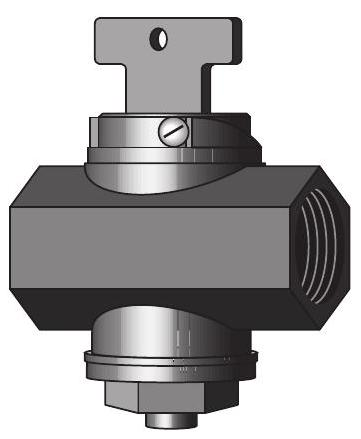
\includegraphics[max width=\textwidth]{CurbStop}

Curb stop

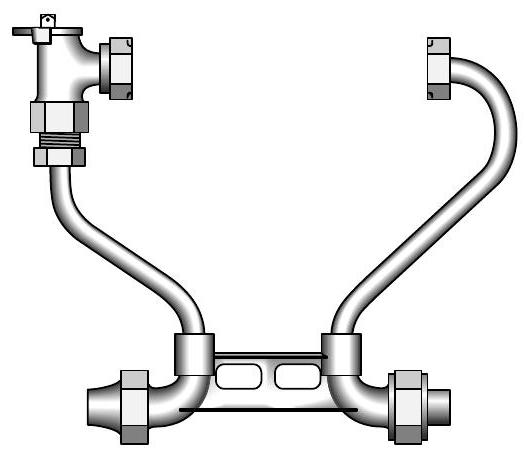
\includegraphics[max width=\textwidth]{MeterSetter}

Meter Setter

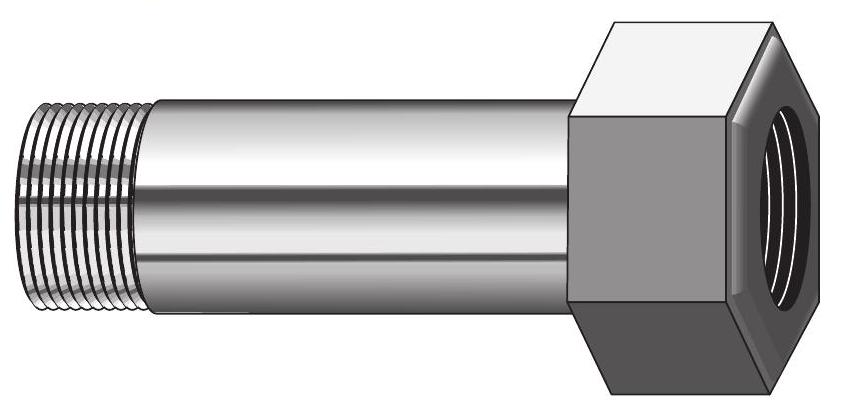
\includegraphics[max width=\textwidth]{TailPiece}

Tail Piece

When the meter is installed in the sidewalk area, a meter box gives access for the meter reader. Boxes are commonly made from cast iron, concrete, and plastic. In some instances, large-diameter insulated PVC pipe with a cast iron lid is used as a meter box.

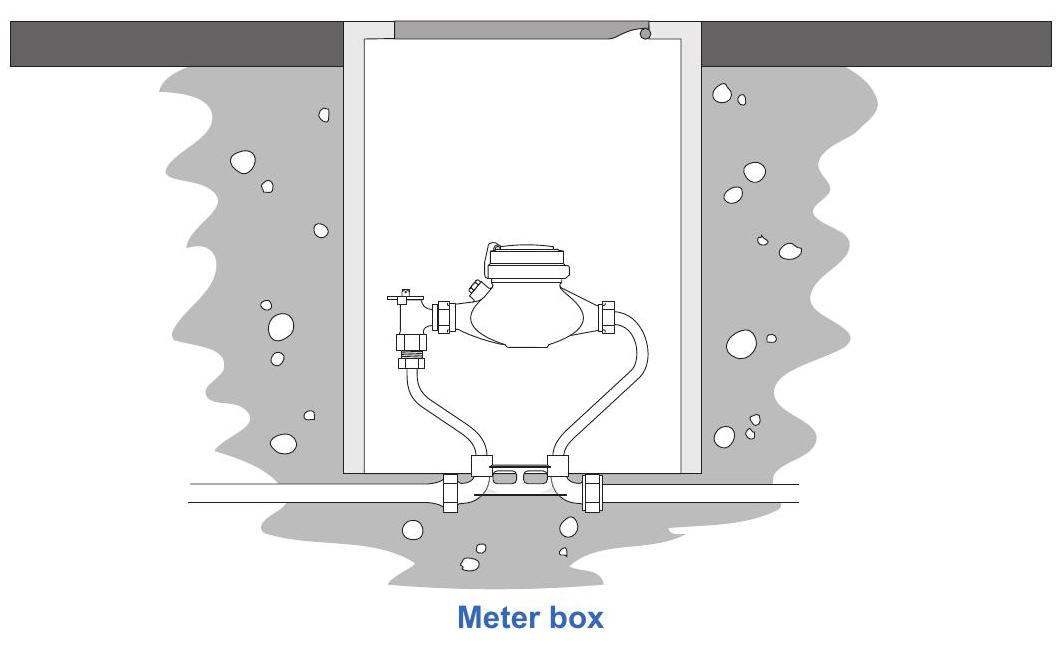
\includegraphics[max width=\textwidth]{MeterBox}

To speed the reading of meters and to make it easier to install meters inside of the house, special meter-reading devices have been developed. These include remote registers that secure to the side of the house or a post and automatic readers that allow the meter reader to obtain the data electronically.

\section{Meter Installations}
The type of meter installation depends upon the environmental conditions of the area. In most of the U.S., a standard meter setting is used. In the Arctic, special circulation systems are required. The most common meter installation is the standard setting. In this setting, a single service line is run from the corporation stop to the meter or from corporation stop to the curb stop and then to the meter.

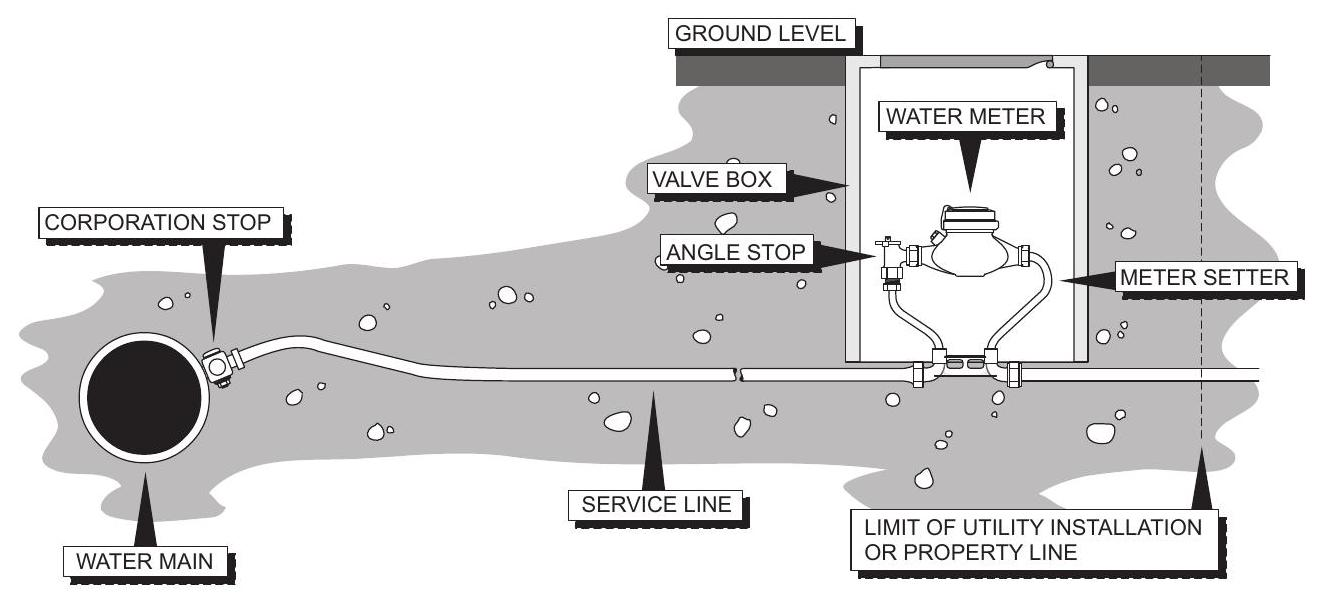
\includegraphics[max width=\textwidth]{MeterBoxInstallation}

Meter box installation

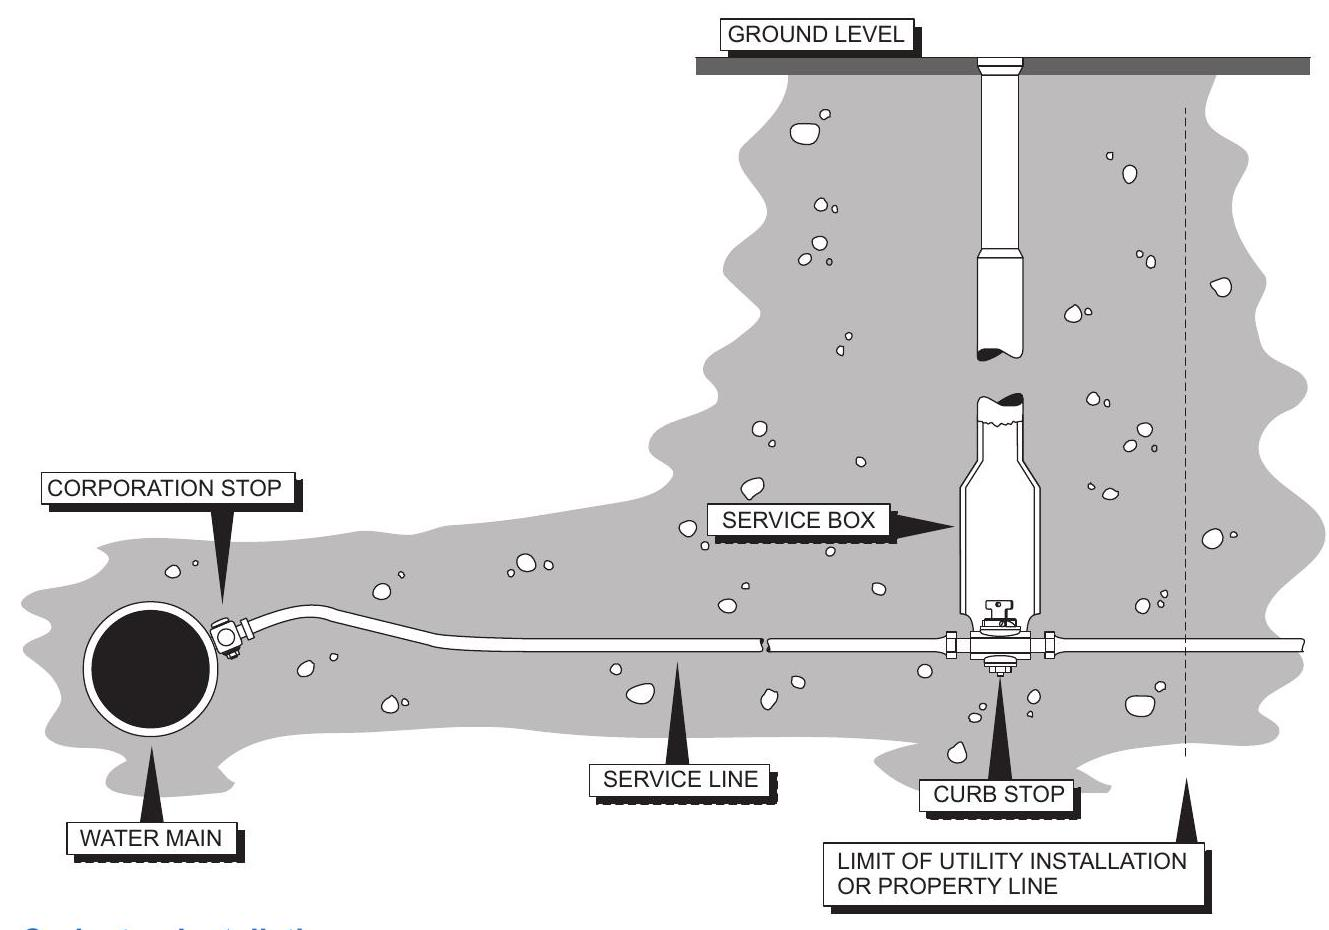
\includegraphics[max width=\textwidth]{CurbStopInstallation}

Curb stop installation

\section{Finished Water Storage}
\section{Function}
There are at least six functions that a storage reservoir can serve in a water distribution system:

\begin{enumerate}
  \item Maintain pressure on the system - In many systems, the elevation of the reservoir determines the pressure in the system.

  \item Provide flow during peak demand ${ }^{21}$ - In many water systems, it is not economical to construct a treatment facility or well that has large enough capacity to meet the peak hourly or daily demand. The water in the reservoir can be drawn into the system to satisfy these peaks.

  \item Provide fire demand.

  \item Provide surge relief - To reduce the surge associated with stopping and starting pumps, systems can be designed so that the pump discharges directly into a reservoir.

  \item Level out pumping demand - To keep pumps from running 24 hours a day, systems are often designed to allow the pumping system to fill the reservoir to a specific level. The pumps then shut off, and water is drawn from the reservoir until the level drops to a predetermined point at which time the pumps restart.

  \item Provide or increase detention time - This is done to provide chlorine contact time and satisfy the desired $\mathrm{CT}$ values requirements.

\end{enumerate}
\section{Reservoir Types}
There are four basic types of reservoirs:

\begin{itemize}
  \item Built with all or most of the reservoir below ground

  \item Built at ground level

  \item Elevated above the ground (elevated tanks or standpipes)

  \item Hydropneumatic tanks (tanks that are pressurized with air)

\end{itemize}
\section{Steel Tanks}
One of the materials used to construct reservoirs is steel. There are two types of steel tanks: welded and bolted. Because of cost, the bolted tanks are the most common in rural Alaska. Steel tanks are typically installed above ground or elevated. Elevated tanks are also called standpipes. Steel tanks are placed on a concrete pad or on an oilsoaked sand pad. The oil reduces deterioration of the bottom of the steel tank.

\section{Concrete Tanks}
There are two types of concrete tanks:

\begin{itemize}
  \item Cast-in-place tanks are installed below ground or above ground. The concrete is poured into forms much like the walls of a home basement, but with more reinforcement.

  \item Prestressed tanks are commonly installed above ground. A prestressed tank is made by wrapping a wire or cable tightly around the tank, stressing the concrete. This wire is covered with concrete to prevent deterioration. The concrete in a prestressed tank is in a relaxed condition when the tank is full. This commonly extends the life of the tank. ${ }^{21}$ Peak Demand - the maximum momentary flow required for a water treatment plant, pumping station or distribution system. The demand is usually the maximum average flow in one hour or less.

\end{itemize}
\section{Wood Tanks}
In many rural areas, including southeast Alaska, wood reservoirs are very common. The insulation capabilities of the wood, along with the low cost of construction, make wood a good choice for the small community. The most common wood tanks are made from vertical tongue-and-groove Douglas Fir or Redwood slats. The slats are held in place by steel bands, which may be galvanized or covered by polyethylene to prevent rusting.

One of the major operational problems with wooden tanks is preventing bacteria that are already in the wood from causing positive bacteriological samples. Special cleaning and chlorination practices are required to reduce this problem.

Wood tanks are installed with either wood or concrete floors. Concrete floors are poured directly on compacted soil. Wood floors are protected from the ground by being installed on concrete or wood pilings.

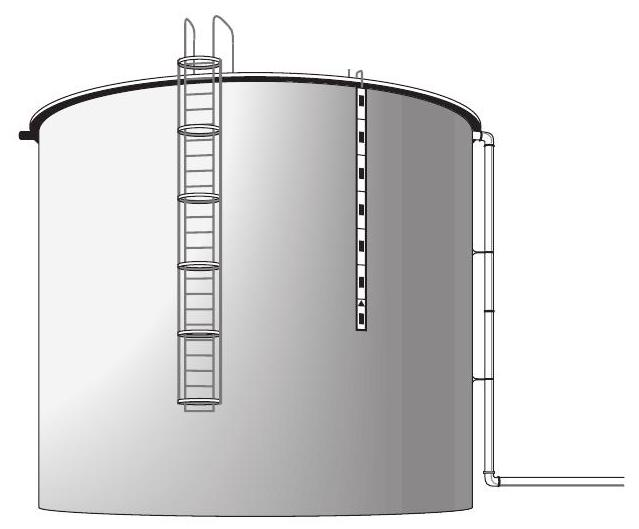
\includegraphics[max width=\textwidth]{2022_11_03_fc0cbc2f3612fab6edd2g-30}

Steel tank

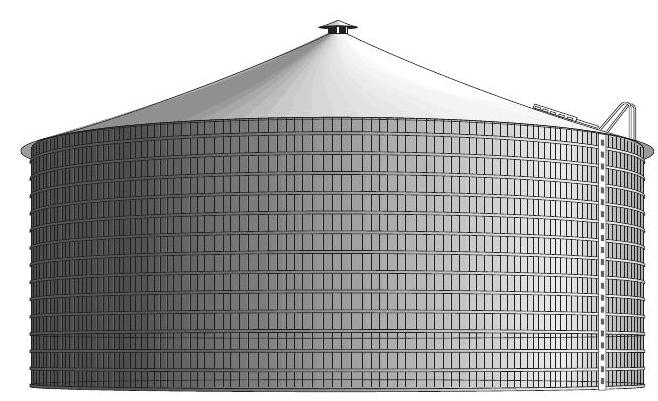
\includegraphics[max width=\textwidth]{2022_11_03_fc0cbc2f3612fab6edd2g-30(1)}

Wood reservoir (storage tank)

\section{Hydropneumatic Tanks}
Hydropneumatic tanks, or pressure tanks, are constructed of steel or fiberglass. These tanks are pressurized by a pump or a pump and air compressor. The tanks commonly contain $1 / 3$ air and $2 / 3$ water. The air is compressed when the tank is filled, acting like a big spring. When the pump shuts off, the air is used to push the water out of the tank.

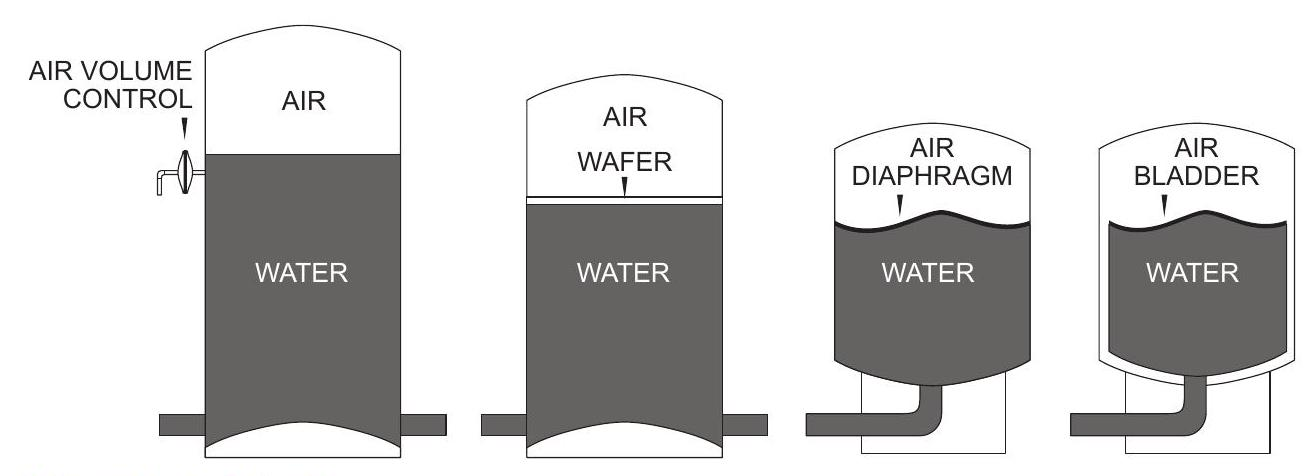
\includegraphics[max width=\textwidth]{2022_11_03_fc0cbc2f3612fab6edd2g-30(2)}

Hydropneumatic tanks

\section{Valves and Piping}
The reservoir water level is controlled by one or more of several popular techniques, each of which control the flow into the tank:

\begin{itemize}
  \item Float valves - A float valve works very much like the float in a toilet bowl and can be installed on the inlet line. As the level of water in the tank changes, the position of the movable closure in the valve changes, which adjusts the amount of water flowing into the reservoir.

  \item Electric controls - Electric controls include electrodes, floats, pressure switches, and sonic devices used to sense the level of water in the reservoir and turn a pump on or off. They can also be used to operate chemical feed pumps.

  \item Altitude valves - These are commonly wide body globe valves. The valve senses the water level in the tank by one of many techniques. A signal, associated with the water level, is sent to the chamber on top of the valve. This changes the position of the movable closure.

  \item Isolation - Regardless of the type of inlet control system, each reservoir must be equipped with an isolation valve on the inlet. This may be a butterfly or gate valve.

\end{itemize}
\includegraphics[max width=\textwidth]{2022_11_03_fc0cbc2f3612fab6edd2g-31}

The outlet normally extends a few inches above the floor to prevent silt, which may enter the tank, from flowing out of the tank. The outlet is commonly screened and includes some type of isolation valve.

The drain line should be installed at floor level to allow complete drainage and cleaning of the tank. To prevent rodents from entering the drain, a screen or flap gate is installed at the end of the drain line.

The inlet and outlet piping (and sometimes baffling) should be installed to minimize short-circuiting when using the reservoir for chlorine contact time.

It is important that each reservoir be installed with some type of by-pass piping and valving. This allows the reservoir to be taken offline for cleaning without interrupting service to customers.

\section{Auxiliary Equipment}
One of the methods used to prevent the interior of a steel tank from deteriorating due to corrosion is to install a protective system called cathodic protection. Sacrificial zinc anodes are placed in the water and a direct current applied to the anodes. This assures that the current flow through the tank is in a direction that will cause the anodes, not the tank, to deteriorate. The zinc placed on an outboard motor to reduce corrosion is an example of this process.

The entrance hatch should be in a position so that it is easy to access. To reduce the possibility of unauthorized entry and possible contamination, the hatch should remain locked except when in use. The best hatches are of the "shoe box" design, where the lid overlaps the hatch opening. This prevents rain from entering the reservoir.

\section{Confined Space}
A storage reservoir is a confined space. Entry for inspection should only be done in accordance with the confined space entry requirements.

Ladders are installed on the outside of the tank to allow access to the hatch. These ladders are usually locked, or access is restricted by raising the end of the ladder several feet above the ground to deter vandalism. The ladder on a storage reservoir may require special fall protection to prevent injury.

To reduce access to the reservoir, it is common practice to surround the reservoir with a six-foot-high chain link fence with a gate that remains locked, except when maintenance is being performed on the tank.

To prevent the collapse of a reservoir when all of the water is drawn out, one or more vents are installed. These vents should be screened to prevent the entrance of birds, rodents, and insects.

A storage reservoir is a confined space. Entry into this space requires that you follow the confined space entry permit requirements. When spraying a chlorine solution, you should wear chemical safety goggles, a cartridge respirator, rubberized gloves, and protective clothing.

\section{Cold-Climate Distribution Systems}
\section{Utilidors}
Utilidors are used in some arctic locations to house and protect water distribution and sewer collection systems. The utilidor also provides access for maintenance to piping, valves, and fire hydrants.

There are three types of utilidors - those made with concrete, those made with wood, and those made with arctic pipe:

\begin{itemize}
  \item Concrete utilidors - Concrete utilidors are usually installed underground, such as in Fairbanks. Concrete utilidors are not very common because of their cost. They usually contain a large variety of utilities such as water, sewer, electricity, phone, TV cable, and commercial heat.

  \item Wood utilidors - Wood utilidors are more popular than concrete, but still not very common. The cost of construction is their major disadvantage. There are two types of wooden utilidors: those constructed of plywood and insulated on the inside with high-density polyurethane or polystyrene and those made of laminated planks and insulated on the outside, such as in Barrow. Wood utilidors can be installed above or below ground. One of the major problems with below-ground utilidors is flooding from a water or sewer line failure or leakage from the outside during spring and summer months.

  \item Arctic pipe utilidors - Among the most common utilidor systems are those made with arctic pipe. Standard arctic pipe made with PVC or HDPE carrier and 16-gauge corrugated steel coating is used. The water line is laid inside of the carrier. The carrier may also contain sewer lines and heating lines or heat trace tape. Arctic pipe utilidors may be installed above or below ground.

\end{itemize}
Utilidors are commonly heated with a hot water or a glycol loop from a low-pressure boiler and heat exchanger, from a forced air heating system, or from self-regulating heat trace tapes.

\section{Arctic Pipe}
Arctic pipe is a general name given to piping material that is made of three components:

\begin{itemize}
  \item An inside pipe, called a carrier

  \item Several inches of high-density polyurethane or polystyrene insulation that protects the carrier

  \item An outside protective layer

\end{itemize}
The most common carriers are made of PVC or HDPE. The outside cover can be made from a variety of materials. The two most common are polyvinyl chloride butyl rubber and 16-gauge corrugated steel or aluminum. The polyvinyl chloride butyl rubber coating is commonly used in underground installations, and the corrugated steel is the most commonly used in above-ground installations.

Arctic pipe can be purchased with a built-in heat trace tape designed to prevent freezing in extreme conditions. This tape can be installed in the field or at the factory. The tape is placed against the carrier, and electrical connections should be made at each joint.

\includegraphics[max width=\textwidth]{2022_11_03_fc0cbc2f3612fab6edd2g-33}

Arctic pipe

Size is relative to the component being discussed. The arctic pipe industry makes insulated pipe from all of the popular materials and in the ranges normally manufactured. In Alaska's rural communities, the most common carriers are 160 psi, two inches through six inches HDPE. Insulation thickness varies from one to three inches, depending on the expected temperature around the pipe. As mentioned earlier, the exterior material varies from a 20 mil laminated polyvinyl chloride butyl rubber coating to 16 -gauge steel or aluminum.

\includegraphics[max width=\textwidth]{2022_11_03_fc0cbc2f3612fab6edd2g-34}

Arctic pipe with heat trace system

The joints for the carrier are made in the same manner as if the carrier were not associated with the arctic pipe. The joints for the polybutyl cover are made by installing insulation, wrapping the insulation with the tape, and covering the tape with an epoxy. Joints for the corrugated cover are made by use of a split cover that is placed around the joint and bolted together.

\section{Circulation Systems}
Many arctic water distribution systems are designed with circulating water mains constructed as loops. The water may be heated to a temperature above freezing ( 40 to $45^{\circ} \mathrm{F}$ ) by means of a heat exchanger at the water treatment plant and then pumped through a service area zone and returned to the treatment building. Oil-fired, lowpressure, hot water boilers are a common source of energy for the heat exchanger. If a water-glycol mixture is used for the exchanger, propylene glycol that is non-toxic should be used.

In the circulation system, there are two taps and two lines: an entry line and a return line. The corporation stops are the pitorifice type. This device is a standard corporation stop with a Pitot tube bend on the inlet. The inlet pitorifice is pointed into the flow, and the outlet pitorifice is pointed away from the flow. The service line loops into and out of the house. If there is a meter, it is attached to a tee on the top of the loop. In some instances, a small pump is installed in the service line to assure constant movement. In order for the pitorifice to work properly, the service line cannot be over 60 feet in length, and the velocity in the main line must be at or above two feet per second (two ft/sec).

\includegraphics[max width=\textwidth]{2022_11_03_fc0cbc2f3612fab6edd2g-35}

Dual pitorifice installation designed to assure continuous circulation of water

Heat trace tape is occasionally installed in conjunction with circulating systems.

If the meter is installed using copper piping, a wire with clips must be placed across the meter before the meter is removed. This protects the operator in case the electrical system is grounded to the water system.

Service connections from the utilidor to the customer are made using arctic pipe containing all of the services. The arctic pipe is sealed to the utilidor.

To reduce the potential of water freezing in them, steel tanks are often covered with three inches of polystyrene or polyurethane boards or spray. The insulation is then covered with metal or fiber coating to protect the insulation from damage.

\section{Cold Weather Operation}
A common problem in arctic environments is frozen water lines. There are three acceptable methods used to thaw these lines.

\section{Electrical}
While electrical thawing has been used to thaw frozen steel and copper lines, its use is discouraged. For quite some time, it has been recognized that electrical thawing of water mains can be quite dangerous. Many communities no longer allow metal utility pipe for use as a ground. There have been instances where if the voltage and amperage are not controlled, home circuits may be damaged or destroyed, and, in extreme cases, the entire home may be destroyed by fire. The popular use of HDPE and PVC pipe do not lend themselves to electrical thawing. The exception to this rule are plastic pipelines installed with a heat-tracing conductor suitable for maintaining flow and thawing if feasible.

\section{High Pressure}
One of the common effective methods of thawing small diameter lines is with the use of a high-pressure washer or jet unit. This device produces a pressure of $2200 \mathrm{psi}$ at a flow of $5.2 \mathrm{gpm}$. The water can be heated with an inline heater to $50^{\circ} \mathrm{F}$ to $180^{\circ} \mathrm{F}$. The water is pumped at high pressure through a small-diameter line that is hand-fed into the frozen line. The pressure and heat are used to thaw the line. This unit has been effective at temperatures as low as $-10^{\circ} \mathrm{F}$.

\section{Steam}
A steam unit, similar to the high-pressure unit, is also commonly used to thaw water lines. A positive displacement pump is used to pump $500^{\circ} \mathrm{F}$ steam at $1.5 \mathrm{gpm}$ through a small line. The small line is hand-fed into the frozen pipe. The steam is produced by an oil-fired boiler that uses kerosene or No. 1 fuel oil. Steam should not be used on plastic or HPDE pipe unless the temperature can be reduced to under $230^{\circ} \mathrm{F}$.

\section{Hot Water}
In many cold-climate regions, a hot water technique is used to thaw frozen water mains and services. This may be done by breaking the service in the home and feeding a $1 / 4$ to 3/16-inch tube into the service line. The tube is advanced to the point of blockage, and then hot water is fed through the tube as it advances until the blockage is melted. Since this procedure may form a cross connection with the potable water system, action must be taken to protect the public supply by using disinfected water or a backflow assembly.

\section{Operation and Maintenance of Distribution Systems}
The proper $\mathrm{O} \& \mathrm{M}$ of distribution systems is part of the overall $\mathrm{O} \& \mathrm{M}$ of the water facility and includes the following activities:

\begin{itemize}
  \item Collecting bacteriological samples

  \item Testing for chlorine residuals

  \item Finding and repairing leaks

  \item Testing system pressure at various locations on a systematic basis

  \item Flushing the main lines at least once a year

  \item Inspecting fire hydrants twice a year (fall and spring)

  \item Locating and exercising in-line valves at least once a year

  \item Cleaning the storage reservoir once a year

  \item Inspecting the storage reservoir, screens, valves, and hatches once a year

  \item Replacing pilot valves and valve seats and inspecting the main valve seat on all pressure-reducing valves and altitude valves once a year.

\end{itemize}
\section{Water Distribution System Quality}
The following is the six-Step program for maintaining "Good" water in the distribution system:

\begin{enumerate}
  \item Maintain a positive pressure of at least 20 psi.

  \item Manage the "age" of the water.

  \item Maintain a chlorine (or other disinfectant) residual.

  \item Keep the pipelines clean.

  \item Provide treatment so that the water does not degrade in the water distribution system.

  \item Set up Water Quality Goals, and test the water frequently. The minimum pressure should be $20 \mathrm{psi}$ throughout the distribution system. If the pipelines are designed to carry fire flow, the 20 -psi minimum pressure should be maintained at the location of the fire, plus all service points in the system during the fire. Care should be used when opening and closing fire hydrants because a surge may cause a drastic fluctuation in high and low pressure in the system. Hydrants valves should always be turned SLOWLY.

\end{enumerate}
Manage storage tanks and pumps to reduce the age of the water and keep the water moving in the distribution system as much as possible. Water should not sit stagnant in the system for more than five days. Water movement can be improved by eliminating dead-end pipes and re-configuring pressure zones. Dead-end water mains are often the source of taste and odor complaints from customers.

Often, storage tanks are oversized to provide fire protection or water for future growth. Water may fail to "turnover" in the tank because of low flow or layering due to temperature differences. Reservoir turnover can be improved by changing the drawdown levels in the tank to draft more water or by adding a recirculation pump. When tank water level controls are altered, system pressure should not be decreased below minimum levels. Additionally, some tanks may have been designed to meet chlorine contact time using a set volume. Good mixing of water can be achieved in a tank by using a small recirculation pump, turbulent inflow, diffusers, or all three of these methods.

Regulations typically require that only a trace of chlorine residual be maintained in the distribution system, but a recordable quantity, such as $0.2 \mathrm{mg} / \mathrm{L}$ measured as a free residual, is suggested throughout the system including dead-end lines.

Pipelines can be maintained in a "clean" condition by removing particles or sediment through adequate treatment prior to distribution. Before a new water main is placed into service, it should be flushed and disinfected and flushed again per AWWA standards. The rehabilitation and repair of water mains are common activities that pose a risk of contamination if not performed properly. Main breaks should be isolated and backflushed to remove debris, then disinfected and tested for coliform before being placed back into service. Along with cleaning, pigging and routine flushing of water mains, a good maintenance program, includes scheduled replacement of old, deteriorated piping.

Flushing may include conventional or unidirectional methods:

\begin{itemize}
  \item Conventional flushing consists of random drawing of water from hydrants without associated valve isolation. The direction of water flow and velocity are not controlled. Deposits may be stirred up, and some are removed, but other sediment may only be moved to another point in the pipeline.

  \item Unidirectional flushing requires prior planning of sequential valve and hydrant operation to move water from the source out toward the extremities of the system. The operator controls water flow and velocity. Velocity is sufficient to remove sediment and biofilm from the pipe interior. The process may include several measurements, such as velocity, chlorine residual, $\mathrm{pH}$, turbidity, and coliform or TTHM sampling. A typical two-person crew can flush one mile of pipeline in an eight-hour shift.

\end{itemize}
Treatment of the water source prior to distribution may be necessary not only to meet turbidity and coliform standards, but also as a means to reduce chlorine demanding substances that could lead to TTHM and HAA5 formation. Often the source water must be treated to reduce its corrosiveness or to remove taste and odor. Consideration should be given to flushing water mains late at night to lessen traffic disruption and minimize customer complaints.

Water quality monitoring goals may include system-wide standards for heterotrophic plate count, chlorine residual, turbidity, taste and odor, or color. Often customer complaints are tracked as a means of better understanding distribution system water quality.

\section{Leak Detection}
In many water distribution systems, a significant percentage of water is lost while in transit from treatment plants to consumers. Recent technical publications indicate that the amount of lost or "unaccounted for" water is typically in the range of 20 to 30 percent of production. Although unaccounted for water is usually attributed to several causes, including leakage, metering errors, and theft, leakage is the major cause. In addition to environmental and economic losses caused by leakage, leaky pipes pose a public health risk, as leaks are potential entry points for contaminants if a pressure drop occurs in the system.

To minimize public health risks and conserve water or save on treatment costs, operators and managers may want to implement leakage control programs. There are two major steps in any systematic leakage control program:

\begin{itemize}
  \item Water audits - Water audits involve detailed accounting of water flow into and out of the distribution system or parts of it. The audits help to identify areas having excessive leakage. Unfortunately, they do not provide information about the location of leaks. To do so, leak detection surveys must be undertaken.

  \item Leak detection surveys - In leak surveys, the water distribution system is checked for leaks by using acoustic equipment that detects the sound or vibration induced by water as it escapes from pipes under pressure. Acoustic equipment includes listening devices, such as listening rods, aquaphones (or sonoscopes), and geophones (or ground microphones). These are used to listen for leak sounds at contact points with the pipe, such as fire hydrants and valves. Acoustic equipment also includes leak noise correlators. These are modern computer-based instruments that have a simple field setup and work by measuring leak signals (sound or vibration) at two points that bracket a suspected leak. The position of the leak is then determined automatically based on the time shift between the leak signals calculated using the crosscorrelation method. Several makes of acoustic leak detection equipment are now commercially available.

\end{itemize}
When water main breaks occur, valves are used to turn off the water so that repairs can be made. If the valves closest to the main break are inoperable, other valves must be closed, necessitating the interruption of water service to additional customers. To reduce the likelihood of this occurring, a water distribution system should be surveyed to determine where older valves should be replaced and where the installation of additional valves would enhance system control. It is recommended that all water distribution system valves be exercised by turning them completely on and off at least once each year. The operator may want to keep precise records of valve loca- tion, age, and maintenance performed, as well as the number of turns needed to open and close the valve.

In most areas, fire hydrants require annual inspections and maintenance. They normally have only a one-year warranty, but some have five-year warranties. These inspections are generally performed by the local utility, but they often do not inspect hydrants identified as private. Fire hydrant manufacturers recommend lubricating the head mechanism and restoring the head gaskets and "O" rings annually so that the fire hydrant can perform the service expected of them. Lubrication is generally done with a food-grade, non-petroleum lubricant to avoid contamination of the distribution system.

Occasionally, a stone or foreign object will mar the seat gasket. In this case, most hydrants have a special seat wrench that allows for removing the seat to replace the gasket or other broken parts without removing the hydrant from the ground. Hydrants extensions are also available for raising a hydrant if the grade around the hydrant changes. Without extending the height, the wrenches to remove caps will not clear, and the break flanges for traffic models will not be located correctly. Hydrant repair kits are also available to repair sacrificial parts designed to break when hit by a vehicle.

Many departments use the hydrants for flushing out water line sediments. When doing so, they often use a hydrant diffuser, which is a device that diffuses the water so that it doesn't damage property and is less dangerous to bystanders than a solid stream. Some diffusers also dechlorinate the water to avoid surface water contamination.

\section{Storage and Reservoir Inspection and Maintenance}
Reservoir cleaning, leak testing, and inspection are ways to assure the integrity of a utility's water storage facilities and to preserve overall water system reliability. Many water systems have adopted procedures from the American Water Works Association (AWWA) for inspecting steel tanks, standpipes, and reservoirs. The only exceptions are those facilities that cannot be removed from service without jeopardizing public health and welfare.

Tanks and reservoirs should be inspected externally and leak-tested annually. Primary reservoirs should be cleaned and disinfected every three years. All other reservoirs should be cleaned and disinfected every five years. Interior inspection should be no fewer than every five years, or whenever routine cleaning and disinfection is completed. After cleaning, if the reservoir was drained, it should be disinfected by spraying the walls with a five percent chlorine solution. If the reservoir is full of water, sufficient chlorine may be added to bring the residual to $10 \mathrm{mg} / \mathrm{L}$ for a 24-hour holding period.

Leakage test results and applicable reservoir or tank inspection information may be documented on a reservoir inspection form, signed, dated, and kept in a permanent maintenance file. This form should note the condition of interior paint or coating, interior pitting or cracking, any repairs made, and the condition of structural components.

\section{Review}
\begin{enumerate}
  \item Arctic pipe is composed of three components. Name these three components.

  \item What gauge metal is used on the outside of arctic pipe?

  \item What standard pipe sizing is used for the OD of HDPE pipe?

  \item What is a pitorifice?

  \item Describe two methods of heating a utilidor.

  \item Describe three methods for thawing frozen water lines.

\end{enumerate}
\section{Cross Connection Control}
${ }^{22}$ Seal Water - The water supplied to the stuffing box to lubricate and flush the packing or the mechanical seal. ${ }^{23}$ Cross connection - Any physical arrangement whereby a public water supply is connected, directly or indirectly, with a non-potable or unapproved water supply or system.

\section{Health Risk}
The plumbing at schools, water treatment plants, wastewater plants, and other public and private facilities can be so complicated that the potable water piping can be unintentionally connected to a source of contamination. If this happens, a health risk is created. There are hundreds of incidents each year where contaminated material enters a water system through cross connections.

In small communities, possible sources of contamination are associated with swimming pools and wastewater treatment plants where chemicals such as chlorine, fluoride, and boiler additives are used.

A health risk can exist if the drinking water system is connected directly or indirectly to contaminated sources. This can happen when a chemical is mixed and the hose is placed in the mixing tank or the drinking water system is connected to the seal water $^{22}$ supply on a sewage pump. This direct or indirect connection is called a cross connection ${ }^{23}$.

The cross connection can only cause a problem if there is a reversal of flow in the system. This reversal of flow is called backflow. Backflow exists anytime water moves backward through the system.

There are two ways that backflow can occur:

\begin{itemize}
  \item Backsiphonage occurs when the pressure in the system drops below atmospheric pressure and the water distribution system is connected to a nonpotable source that is open to the atmosphere. This can happen if the distribution system pressure is lowered as a result of a main break or heavy use, such as during a fire. - Backpressure exists any time the pressure in the contaminated source exceeds the pressure in the distribution system. This can happen as a result of a booster pump in a heating system or excessive pressures in a boiler improperly connected to the potable water supply.\\

\includegraphics[max width=\textwidth]{2022_11_03_fc0cbc2f3612fab6edd2g-41}${ }^{24}$ Double Check Valve Assembly - An assembly of two independently acting check valves with shut-off valves on each side of the check valves and test ports for checking the water tightness of each check valve. ${ }^{25}$ Air Gap - A positive means of preventing a cross connection. An air gap should be twice the diameter of the discharge pipe or a minimum of $\mathrm{I}$ inch above the rim of the tank. Each state's drinking water regulations indicate that a known cross connection cannot be allowed to exist. Because inspection of facilities is difficult, time-consuming, and not always possible, the waterworks industry has taken a preventive approach to cross connection control. Under this approach, facilities that have a high potential of cross connection or that handle highly hazardous materials are required to protect the water system. This is accomplished by installing special devices in the facility and on the water service connection where it enters the facility.
\end{itemize}
\section{Assemblies}
The assemblies used to prevent backflow from a potential cross connection include the following:

\begin{itemize}
  \item Air gaps

  \item Atmospheric vacuum breakers

  \item Pressure vacuum breakers

  \item Double check valve assemblies ${ }^{24}$

  \item Reduced pressure zone backflow prevention assemblies

\end{itemize}
The assembly to be used should be selected based upon the degree of hazard, plumbing arrangement in the facility, and the use of additional devices within the facility.

A high-hazard facility would include a sewage treatment plant or lift station. A low level of hazard would be a situation where the odor and taste of the water might be affected, but there is no health risk.

The most protective of the assemblies is the air gap $^{25}$. The air gap is easy to observe and inspect. The air gap is a positive way to protect the water supply from a chemical vat. The requirements are that the air gap between the two water sources be twice the diameter of the outlet of the supply line but no less than one inch from the rim of the tank. Air gaps can be used on high-hazard conditions.

Atmospheric vacuum breakers are used on low-degree

\includegraphics[max width=\textwidth]{AirGap}\\
hazard conditions, such as janitor sinks, lawn sprinkler systems, and supply lines on low-concentration chemical vats, such as chlorine and fluoride solutions. Atmospheric vacuum breakers open any time there is a backsiphonage and allow air to be drawn into the line, preventing a

${ }^{26}$ Vacuum Breaker - A mechanical device that prevents backflow due to siphoning action created by a partial vacuum that allows air into the piping system, breaking the vacuum. backflow of the downstream solution. They will not prevent backflow as a result of backpressure. A downstream valve cannot be installed on an atmospheric vacuum breaker ${ }^{26}$.

\includegraphics[max width=\textwidth]{AtmosphericVacuumBreaker}

Atmospheric vacuum breaker

\includegraphics[max width=\textwidth]{PressureVacuumBreaker}

Non flow condtions Pressure vacuum breakers are used for the same functions as an atmospheric vacuum breaker. There are only three differences:

\begin{itemize}
  \item The pressure vacuum breaker has an internal spring that helps it to open.

  \item There are valves to allow the assembly to be tested.

  \item A valve can be placed in the downstream line.

\end{itemize}
They are not designed for connections where backpressure may exist.

A double check valve assembly (DCVA) is composed of two independent internally weighted check valves (springs), isolation valves on each side of the assembly, and test ports on the assembly that allow a tester to determine that the check valves are watertight. DCVAs protect against backpressure or backsiphonage on low-hazard conditions.

\includegraphics[max width=\textwidth]{DoubleCheckValveAssembly}

High-hazard conditions require an air gap or a reduced pressure zone backflow prevention assembly $(\mathrm{RPZ})^{27}$. It is composed of two independent, internally weighted check valves separated by a reduced pressure zone valved to the atmosphere. The assembly also has an isolation valve on each end, as well as test ports to determine the proper operation of the assembly. The valve is designed so that the valve on the reduced pressure zone will open when the pressure in the zone gets to within two psi of the supply pressure. For backflow to occur through this valve, the two check valves, as well as the reduced pressure zone valve, would all have to fail at the same time.

\includegraphics[max width=\textwidth]{RPZBFPA}

${ }^{27}$ RPZ (Reduced Pressure Zone Backflow Prevention Assembly) -A backflow prevention assembly containing two check valves, a differential relief valve located between the two check valves, shut-off valves on each end of the assembly, and test ports for checking the water tightness of the check valves and the operation of the relief valve. Only approved assemblies may be installed in a water system. For an assembly to be approved, it must undergo extensive testing by a private testing laboratory. ADEC maintains a listing of approved assemblies. Contact the regional ADEC representative for a listing of these devices.

A certified backflow prevention device tester must test the assemblies once each year. To obtain a certification as a backflow prevention assembly tester, you must attend a school and pass a written and practical exam. To maintain your certification, some states require an annual refresher course, proof that you have tested devices in the past year, and a certificate indicating that your test instruments have been tested within the past year.

\section{Review}
\begin{enumerate}
  \item Describe the terms backsiphonage and backpressure.

  \item Name the proper cross connection control device for a sewage treatment plant, clinic, and a boiler feed water to a glycol system.

  \item Cross connection control devices should be tested how often?

\end{enumerate}
\section{Water Distribution Systems Quiz}
\begin{enumerate}
  \item Which of the following primarily determines the size of water mains, pumping stations, and storage tanks?\\
A. Maximum day demand during the 24-hour period during the previous year\\
B. Population served\\
C. Per-capita water use\\
D. Fire protection requirements

  \item Which of the following is a measure of the smoothness of pipe?\\
A. S factor\\
B. C value\\
C. Hazen-Williams formula\\
D. T factor

  \item The primary purpose of check valves is to prevent:\\
A. Excessive pump pressure\\
B. Priming\\
C. Water from flowing in two directions\\
D. Water hammer

  \item Why is excessive water pressure to residential homes objectionable?\\
A. Increases particulate matter reaching the customer\\
B. Causes erosion of the copper plumbing due to the high velocities, giving the water a metallic taste\\
C. Decreases the life of the water heaters and other water-using appliances\\
D. Causes foaming from faucets

  \item What is the best time to perform a flushing program on the mains?\\
A. Spring when the weather is usually mild\\
B. Fall when water usage is low and the weather not yet harsh\\
C. Late at night to lessen traffic disruption and minimize customer complaints\\
D. Summer when many residents are on vacation

  \item Large full storage tanks are typically disinfected with a chlorine residual of which of the following?\\
A. $3 \mathrm{mg} / \mathrm{L}$\\
B. $10 \mathrm{mg} / \mathrm{L}$\\
C. $25 \mathrm{mg} / \mathrm{L}$\\
D. $50 \mathrm{mg} / \mathrm{L}$

  \item Which one of the following service line materials is not flexible?\\
A. Copper\\
B. Galvanized iron\\
C. Lead\\
D. Plastic 8. What is the term for a framework of wood or metal installed to prevent caving of trench walls?\\
A. Sheeting\\
B. Sloping\\
C. Shielding\\
D. Shoring

  \item Which type of pipe is typically used in the construction of very large water mains?\\
A. Asbestos-cement\\
B. Steel\\
C. Plastic\\
D. Galvanized

  \item Air-relief valves are installed for which of the following reasons?\\
A. Release some of the energy created by water hammer\\
B. Stop flow completely when the tank is full\\
C. Vent air that has accumulated in the well column while the well is not in use\\
D. Turn off pressure during hydrant main maintenance without disrupting ser- vice to customers

  \item After a new water main is installed and pressure tested, it should be:\\
A. Flushed with clean water for 24 hours and put into service\\
B. Filled with a solution of $25 \mathrm{ppm}$ to $50 \mathrm{ppm}$ free chlorine for at least 24 hours prior to flushing\\
C. Filled with clean water and allowed to sit for five days at full pressure before turning the water into the system\\
D. Photographed so that mapping can be avoided until the system is complete

  \item Which type of hydrant has no main valve but has a separate valve for each nozzle?\\
A. Wet-barrel\\
B. Warm-climate\\
C. Dry-barrel\\
D. Breakaway

  \item Which of the following type of valve is used in maintaining prime to a pump?\\
A. Foot\\
B. Suction\\
C. Vacuum header\\
D. Butterfly

  \item Which of the following metals make the best anode?\\
A. Brass\\
B. Cast iron\\
C. Zinc\\
D. Copper 15. A six-inch pipeline needs to be flushed. If the desired length of pipeline to be flushed is 316 feet, how many minutes will it take to flush the line at $31 \mathrm{gpm}$ ?\\
A. 10 minutes\\
B. 15 minutes\\
C. 30 minutes\\
D. 60 minutes

  \item Why should the operator contact area companies with underground utilities before starting an underground repair job?\\
A. To determine if there have been recent excavations in that location\\
B. To ask the companies to locate and mark the location of their utilities in the area of the repair job\\
C. To determine if they also have excavating to do in the area\\
D. To ask if they will help route traffic while you are doing the repair job

  \item A six-inch pipeline needs to be flushed. If the desired length of pipeline to be flushed is 316 feet, how many minutes will it take to flush the line at $31 \mathrm{gpm}$ ?\\
A. 10 minutes\\
B. 15 minutes\\
C. 30 minutes\\
D. 60 minutes

  \item What is the area of a trench that is $22.4$ feet long and $3.3$ feet wide?\\
A. $26 \mathrm{sq} \mathrm{ft}$\\
B. $74 \mathrm{sq} \mathrm{ft}$\\
C. $143 \mathrm{sq} \mathrm{ft}$\\
D. $187 \mathrm{sq} \mathrm{ft}$

  \item Interior copper tubing is usually joined by:\\
A. Solder\\
B. Flare\\
C. Compression\\
D. Union

  \item Which type of piping is most resistant to corrosion?\\
A. Plastic\\
B. Stainless steel\\
C. Concrete\\
D. Asbestos-cement

  \item What is the minimum contact time when using the chlorine tablet method of disinfecting water mains?\\
A. 6 hours\\
B. 12 hours\\
C. 18 hours\\
D. 24 hours 22. A pipeline that contains reclaimed water should be tinted or painted what color?\\
A. Orange\\
B. Yellow\\
C. Purple\\
D. Red

  \item What is the diameter of a tank with a circumference of $408.2 \mathrm{ft}$ ?\\
A. $31 \mathrm{ft}$\\
B. $130 \mathrm{ft}$\\
C. $260 \mathrm{ft}$\\
D. $1,282 \mathrm{ft}$

  \item Fuel oils, gasoline, and other organic compounds may permeate which type of piping?\\
A. Plastic\\
B. Asbestos-cement\\
C. Fiberglass\\
D. Concrete

  \item Why should isolation valves be installed at frequent intervals in the distribution piping?\\
A. To stop water from flowing backward through a pump that is not in operation\\
B. To throttle flow and maintain a lower pressure in the lower distribution sys- tem zone\\
C. So that air that accumulates at high points in pipes can be automatically vented\\
D. So that small sections of water main may be shut off for maintenance

  \item What water quality problem is most likely to occur at dead-end water mains?\\
A. Dirty water\\
B. Taste and odor\\
C. Milky water due to air bubbles\\
D. Dirty clothes due to manganese

  \item What type of concrete tank is made like a home basement but with more reinforcement?\\
A. Cast-in-place concrete\\
B. Hydraulically applied concrete-lined\\
C. Circular prestressed-concrete\\
D. Prestressed concrete-wire-wound

  \item PVC pipe can use tees, elbows, and other fittings from what other type of pipe?\\
A. Prestressed concrete cylinder\\
B. Ductile iron\\
C. Concrete\\
D. Asbestos-cement 29. What type of ductile-iron pipe joint is quickly assembled and is the least expensive?\\
A. Flanged joint\\
B. Mechanical joint\\
C. Push-on joint\\
D. Ball-and-socket joint

  \item Where is the most common location of leaks on old service connections?\\
A. Household plumbing\\
B. Connections to the curb stop\\
C. Connections to the gate valve\\
D. Pressure regulator

  \item Dry-barrel fire hydrants are used in what type of environment?\\
A. Dry\\
B. Wet\\
C. Freezing\\
D. Hot

  \item The supply or fill hose for a Watering Point System must be tested and approved by:\\
A. The American Water Works Association (AWWA)\\
B. The Association of State Drinking Water Administrators (ASDWA)\\
C. The National Sanitation Foundation (NSF)\\
D. The Society of Professional Engineers (SPE)

  \item Which of the following is the best type valve to use to dampen a water hammer?\\
A. Pressure-relief\\
B. Needle\\
C. Pressure-reducing\\
D. Pinch

  \item Which of the following valves can be used to control pressure?\\
A. Globe\\
B. Butterfly\\
C. Gate\\
D. Plug

  \item Which of the following valves is best to use in throttling flow?\\
A. Globe\\
B. Butterfly\\
C. Gate\\
D. Ball 36. What is the pressure head at a fire hydrant in feet, if the pressure gauge reads 121 psi?\\
A. $52 \mathrm{ft}$\\
B. $86 \mathrm{ft}$\\
C. $141 \mathrm{ft}$\\
D. $280 \mathrm{ft}$

  \item Which of the following types of valve is the best to use for maintaining the water level in a storage tank?\\
A. Altitude\\
B. Tapping\\
C. Butterfly\\
D. Needle

  \item A joint that consists of a rubber gasket and follower ring held to a flange by a row of bolts is called a:\\
A. Bell and spigot\\
B. Caulder coupling\\
C. Mechanical joint\\
D. Victaulic coupling

  \item Water mains should be separated from sewer mains by:\\
A. At least 24 inches vertically and 60 inches horizontally\\
B. A horizontal distance of $10 \mathrm{ft}$ and vertical distance of 12 inches above the sewer main\\
C. A vertical distance of $5 \mathrm{ft}$ above the sewer and $5 \mathrm{ft}$ horizontally\\
D. A PVC curtain at least $6 \mathrm{mil}$ in thickness extending to a depth of $4 \mathrm{ft}$ below the invert of the sewer main

  \item A thrust block or restrained joint should be installed in a water distribution system:\\
A. At a change in direction, size, dead end, or valve and hydrant locations\\
B. At the apex or high point of every water main to prevent water hammer\\
C. Wherever there is a change in velocity head due to friction\\
D. Whenever a wet tap is made at a point between the curb stop and tapping saddle

  \item A special curb stop design used in arctic climates that enhances circulation through a service connection loop to the home is the:\\
A. Recirculating ball valve\\
B. Heat traced curb device\\
C. Arctic insulated curb stop\\
D. Pitorifice

\end{enumerate}

\end{document}